% !TEX root = ln_diss.tex
\graphicspath{{img/ch2/}}
\chapter[Domain decomposition methods]{Domain decomposition methods for large  problems} \label{chap:DD}

The most important limit of numerical full-wave electromagnetic analyzes is the fact computational resources are limited, at least when trying to fit all the problem in memory at a time. Even if one had infinite computational resources, many algorithms, say even the solvers, would be such that it would require a huge amount of times to solve very large problems. 

Nowadays, we refer to \quotes{large problems} to meshes that lead to millions of unknowns, up to several tens of millions. In chapter \ref{chap:FE}, we could solve acceptably a 600,000 unknowns problem in about 2 minutes (Horn antenna in section \ref{sec:Horn}). But notice that it required about 3.1~GB of memory, which can easily fit in modern (low-cost) personal computers. But what would happen if we try to analyze an array of this antenna? The problem, if full-wave solution is still sought for, would be to solve the wave equation in the all the horns connected by a wide radiation bounding box, allowing thus to consider mutual couplings between the antennas. This slightly increases the number of the finite element unknowns that we would have upon multiplying the 600,000 unknowns by the number of antennas. It is evident that we quickly reach the limit on a simple computer. To overcome this problem, parallel processing needs to be considered, devoting the matrix inversion to multiple computers (increasing in such a way the overall physical memory) interconnected through a high speed network. With iterative solvers, even if they require a minimum of memory which is necessary to store the built finite element system, the number of iterations might dramatically grow with the number of unknowns, hence the amount of times required for an acceptable analysis might not be tolerable.

Among the methods developed to increase the computational efficiency of finite element solvers, domain decomposition (DD) methods have found noticeable interest in the last decade.  They allow to analyze a whole problem upon partitioning it and computing solutions for each smaller problem. Then, all the solutions are \quotes{connected} in order to recover the effective solution within the whole domain. Relying on a \textit{divide et impera} scheme, these methods are \textit{de facto} intrinsically parallelizable. In fact, multiple domains can be analyzed contemporaneously on different processors. Another interesting aspect is that, when no cluster of computers is available to scale the problem, each smaller problem or \textit{subdomain} can be tackled faster with direct solvers, one at a time, while keeping in memory only the necessary information to recover the global solution. 

\begin{figure}[ht]
\centering
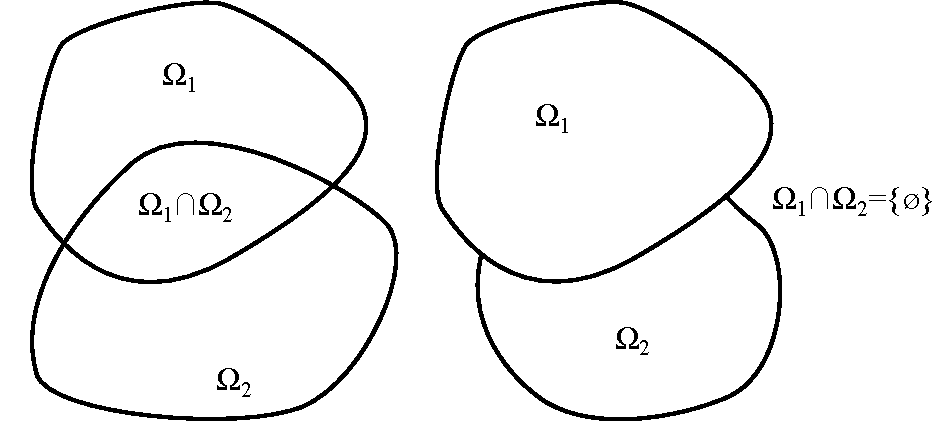
\includegraphics[width=14cm]{DDnonoverlaping}
\caption{Overlaping and non-overlaping domain decomposition schemes.}
\label{fig:DDnonoverlaping}
\end{figure}

A critical part of the domain decomposition method is how the information on the subdomains is collected and transferred to the global problem in order to achieve the original problem solution. There exist in literature \cite{toselli2005domain, mathew2008domain} many mathematically proven algorithms that lead to a domain decomposed solution for a variety of problems (Laplace, Helmholtz, Navier-Stokes and other PDEs) given a particular decomposition scheme. The first domain decomposition algorithm is more than a century old: Schwarz proposed, at the end of $19^\mathrm{th}$ century, an alternating algorithm for the solution of Poisson problems on overlapping subdomains \cite{schwarz1972gesammelte}, proving later its convergence. With the advent of the personal computer, this research field begun to find many interesting applications. The first non-overlapping appeared in 1990 \cite{lions1990schwarz} and has opened the investigation to a new class of domain decomposition algorithms. It is evident, from a computational point of view, how this decomposition scheme is easier to handle. However, new truncation conditions have to be enforced as only the informations on the boundaries can be transferred to the adjacent subdomains.


In this chapter, we investigate two non-overlapping or \textit{iterative substructuring} domain decomposition methods: a Schur Complement based method and a Finite Element Tearing and Interconnecting Dual-Primal (FETI-DP) based method in order to solve large radiation problems either for sequential or parallel computing. In particular, the DD frameworks are employed as preconditionners for iterative solvers for sequential processing. Direct solvers, being the best suited for small problems, can be employed in a DD framework to accelerate the convergence of iterative solvers. Several tests will be performed, first analyzing the performances of the algorithms on an arbitrarily partitioned rectangular waveguide problem.

\section{Schur complement based domain decomposition}\label{sec:SchurDD}

As we have seen in chapter \ref{chap:FE}, the unknowns resulting from a Galerkin framework are somehow related to mesh entities. If one could collect sequentially, during the mapping to the system matrix, the unknowns pertaining to a subdomain, then the resulting matrix would have a block-diagonal form. Of course, the unknowns related to the subdomain boundaries cannot be duplicated, otherwise the resulting system would be undetermined. Thus, one can collect all the unknowns pertaining to the boundaries between subdomains in a new diagonal block. These unknowns, being dependent on the elements pertaining to two (or more) adjacent subdomains, will lead to global matrix entries connected to these subdomains unknowns apart from diagonal blocks.

\begin{figure}[ht!]
\centering
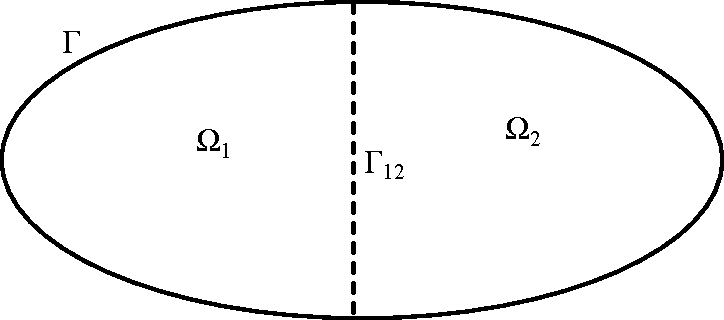
\includegraphics[width=11cm]{DDSchur2}
\caption{Schur complement based domain decomposition sketch for two subdomains.}
\label{fig:DDSchur2}
\end{figure}

Consider the domain decomposition of $\Omega$ in two subdomains as shown in Fig. \ref{fig:DDSchur2}. The resulting system matrix of any formulation employed in chapter \ref{chap:FE} is

\begin{equation}
\label{eq:DDSchurFull}
\begin{bmatrix}
A_{\Gamma\Gamma} & A_{\Gamma1} & A_{\Gamma2}\\
A_{1\Gamma} & A_{11} & \\
A_{2\Gamma} &  & A_{22}
\end{bmatrix}
\begin{bmatrix}
x_{\Gamma}\\
x_{1}\\
x_{2}
\end{bmatrix}
=
\begin{bmatrix}
B_{\Gamma}\\
\phantom{B}\\
\phantom{B}
\end{bmatrix},
\end{equation}

\noindent where the subscript $\Gamma$ refers to shape functions with related mesh entity on $\Gamma \equiv \Gamma_E \cup \Gamma_H \cup \Gamma_R \cup \Gamma_{WG} \cup \Gamma_{12}$, and the subscript $j \in \lbrace 1,2 \rbrace$ refers to unknowns pertaining exclusively to mesh entities in $\Omega_j$. Notice that the right-hand side has only non-zero entries for the formulations employed in chapter \ref{chap:FE}, the Dirichlet boundary conditions corresponding to perfect electric conductors. Furthermore, when isotropic materials are considered (as done almost everywhere throughout this work), the system matrix is symmetric and \eqref{eq:DDSchurFull} can recast in

\begin{equation}
\label{eq:DDSchurSym}
\begin{bmatrix}
A_{\Gamma\Gamma} & A_{\Gamma1} & A_{\Gamma2}\\
A_{\Gamma1}^T & A_{11} & \\
A_{\Gamma2}^T &  & A_{22}
\end{bmatrix}
\begin{bmatrix}
x_{\Gamma}\\
x_{1}\\
x_{2}
\end{bmatrix}
=
\begin{bmatrix}
B_{\Gamma}\\
\phantom{B}\\
\phantom{B}
\end{bmatrix}.
\end{equation}

The system of \eqref{eq:DDSchurSym} can now be solved exploiting the Schur complement concept:

\begin{itemize}
\item Assemble the Schur complement matrix $\mat{S} = \mat{A_{\Gamma\Gamma}} - \sum_{j=1}^2~\mat{A_{\Gamma j}}$ $\mat{A_{jj}}^{-1}~\mat{A_{\Gamma j}}^T$ and the relative right-hand side $\mat{G}~=~\mat{B_{\Gamma}}$,
\item Solve the Schur complement system $\mat{x_\Gamma}~=~\mat{S}^{-1} \mat{G}$,
\item Recover for the internal unknowns $\mat{x_j} = \mat{A_{jj}}^{-1} (-\mat{A_{\Gamma j}}^T \mat{x_\Gamma})$.
\end{itemize}

In the first step, a matrix denser than the original $\mat{A_{\Gamma\Gamma}}$ is assembled upon adding (as done for the global finite element matrix after the computation of an element matrix) the contributions of each subdomain. This requires the computation of $\mat{A_{jj}}^{-1}$ (intrinsically dense), which itself can be handled easily with sparse direct solvers (and exploiting symmetries in this case), however, the computation of the matrix-matrix product $\mat{A_{jj}}^{-1} \mat{A_{\Gamma j}}^T$ may lead to a memory consuming result. Hence, one should consider making the most of $\mat{A_{\Gamma j}}^T$ sparsity to reduce the resulting rectangular matrix, avoiding to save into memory its null column vectors.

The second step corresponds to the inversion of a dense $\mat{S}$ matrix. As it is known, this operation has an asymptotic complexity of $O(N_\Gamma^3)$, which indeed increases as the number of subdomains is increased. In fact, the unknowns on the boundary between subdomains increases. One may solve the problem on boundaries with a Krylov subspace iterative solver, preconditioning it with a \textit{thresholded incomplete LU} factorization  \cite{saad1994ilut} or the \textit{incomplete Cholesky} factorization which takes the advantage of matrix symmetry. In fact, it has been proved \cite{mathew2008domain} that if the original system is symmetric, then the Schur complement matrix will also be symmetric.

The last step requires subdomains matrices inversion. These can be stored in memory (non-volatile preferably) during the first step where they were also used. An additional matrix-vector product has to be computed.

The resulting concatenated solution vector $\vect{x}_\mathrm{Schur} = \vect{x_\Gamma \ x_1 \ x_2}^T$ is equal, within numerical error, to that of the direct solution of the whole system in \eqref{eq:DDSchurSym} when direct or iterative solvers are ran up to numerical precision. Furthermore, the parallelization internal to the first and the last steps is immediate.

In our treatment, several critical points have emerged from the use the Schur complement method, when looking forward to analyze large problems

\begin{itemize}
\item The assembly of the Schur complement matrix requires the computation of large rectangular matrices $\mat{A_{jj}}^{-1} \mat{A_{\Gamma j}}^T$. One may assemble the whole Schur complement to domain $\Omega_j$, $\mat{A_{\Gamma j}} \mat{A_{jj}}^{-1}$ $\mat{A_{\Gamma j}}^T$, upon exploiting the sparsity of $\mat{A_{\Gamma j}}^T$ and considering a few columns at a time in order to reduce the overall memory fill-in. However, if the number of unknowns pertaining to $\Omega_j$ is very large, then this step might result to be excessively time demanding.
\item The overall Schur complement matrix $\mat{S}$ is dense, and the complexity of its inversion grows dramatically with the boundary unknowns, and, consequently, with the number of subdomains.
\end{itemize}

\noindent Both the previous points are in contrast: if one tries to alleviate the computation of the Schur complement matrices to each subdomain by increasing the number of subdomains (hence reducing the related domain unknowns number), then the inversion of the overall Schur complement matrix results hampered by an increase of the boundary unknowns and \textit{viceversa}. This has led to the research of an appropriate Schur complement based domain decomposition preconditionner to be used in an iterative solver for the whole problem \eqref{eq:DDSchurSym}.

In contrast with the method that will be introduced in the next section, Schur complement based methods are referred to as \quotes{primal} iterative substructuring methods in the way they employ only functions in the space of the unknown global function to enforce the continuity between subdomains. For instance, continuity between the subspaces spanned in each subdomain without its boundaries is enforced by a discrete version of the Steklov-Poicar\'e operator or \quotes{Dirichlet-to-Neumann} map \cite{mathew2008domain}, the Schur complement matrix, serving as a mean for continuity of the values and the normal derivatives at the boundaries.

\section[FETI-DP domain decomposition]{Finite Element Tearing and Interconnecting Dual Primal domain decomposition} \label{sec:FETIDD}


Finite element tearing and interconnecting methods where first introduced in 1991 for solving a computational mechanics problem \cite{farhat1991method}. These methods are based on the solution of the subdomains problems with their boundary conditions (tearing) and solving the problem at the boundaries with Lagrange multipliers (interconnecting), the coarse problem which enforces through algebraic constraints the continuity of the global solution at subdomain boundaries. The space spanned by the sough function corresponds to \quotes{primal} unknowns while the space spanned by  the boundary constrains corresponds to \quotes{dual} unknowns.

\begin{figure}[h]
\centering
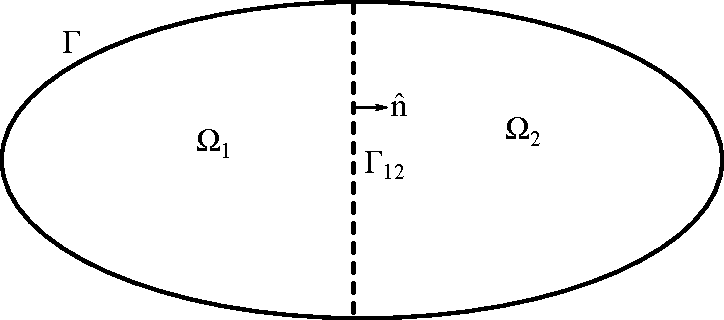
\includegraphics[width=11cm]{DDFETI}
\caption{FETI-DP based domain decomposition sketch for two subdomains.}
\label{fig:DDFETI}
\end{figure}

Let us consider the problem depicted by Fig. \ref{fig:DDFETI}. We seek to solve the following distinct boundary value problems defined as
%
\begin{equation}
\label{eq:FETID1}
\left\lbrace
\begin{aligned}
\nabla \times \frac{1}{\mu_r} \nabla \times {\mathbf{E}^1} + j k_0 \zeta_0 \sigma {\mathbf{E}^1} - k_0^2 \epsilon_r {\mathbf{E}^1} = 0,& \quad \mathrm{in} \ \Omega_1,\\[10pt]
\hat{\mathbf{n}} \times ( {\mathbf{E}^1} \times \hat{\mathbf{n}}) = 0, &\quad \mathrm{on} \ \mathrm{\Gamma}_E \cap d\Omega_1, \\[5pt]
\hat{\mathbf{n}} \times ( {\mathbf{H}^1} \times \hat{\mathbf{n}}) = 0, &\quad  \mathrm{on} \ \mathrm{\Gamma}_{H} \cap d\Omega_1, \\[5pt]
\hat{\mathbf{n}} \times \mathbf{H}^1 = \frac{1}{Z_s} \hat{\mathbf{n}} \times \hat{\mathbf{n}} \times \mathbf{E}^1 + \hat{\mathbf{n}} \times \mathbf{H}^{inc} - \frac{1}{Z_s} \hat{\mathbf{n}} \times \hat{\mathbf{n}} \times \mathbf{E}^{inc}, &\quad \mathrm{on} \ \Gamma_{R} \cap d\Omega_1, \\[5pt]
\hat{\mathbf{n}} \times \mathbf{H}_t^{1,k} = \frac{1}{Z_k} \hat{\mathbf{n}} \times \hat{\mathbf{n}} \times \mathbf{E}_t^{1,k} - \frac{2}{Z_k} \hat{\mathbf{n}} \times \hat{\mathbf{n}} \times \mathbf{E}_t^{k \ inc}, &\quad \mathrm{on} \ \Gamma_{WG}^k \cap d\Omega_1,\\[5pt]
\hat{\mathbf{n}} \times \frac{1}{\mu_r} \nabla \times \mathbf{E}^1 - jk_0 \ \hat{\mathbf{n}} \times \mathbf{E}^1 \times \hat{\mathbf{n}} = \qquad \qquad &\\ - \hat{\mathbf{n}} \times \frac{1}{\mu_r} \nabla \times \mathbf{E}^2 - jk_0 \ \hat{\mathbf{n}} \times \mathbf{E}^2 \times \hat{\mathbf{n}},  &\quad \mathrm{on} \ \Gamma_{12} \cap d\Omega_1, \\[5pt]
\end{aligned}
\right.
\end{equation}
%
\noindent and 
%
\begin{equation}
\label{eq:FETID2}
\left\lbrace
\begin{aligned}
\nabla \times \frac{1}{\mu_r} \nabla \times {\mathbf{E}^2} + j k_0 \zeta_0 \sigma {\mathbf{E}^2} - k_0^2 \epsilon_r {\mathbf{E}^2} = 0,& \quad \mathrm{in} \ \Omega_2,\\[10pt]
\hat{\mathbf{n}} \times ( {\mathbf{E}^2} \times \hat{\mathbf{n}}) = 0,& \quad \mathrm{on} \ \mathrm{\Gamma}_E \cap d\Omega_2, \\[5pt]
\hat{\mathbf{n}} \times ( {\mathbf{H}^2} \times \hat{\mathbf{n}}) = 0,& \quad  \mathrm{on} \ \mathrm{\Gamma}_{H} \cap d\Omega_2, \\[5pt]
\hat{\mathbf{n}} \times \mathbf{H}^2 = \frac{1}{Z_s} \hat{\mathbf{n}} \times \hat{\mathbf{n}} \times \mathbf{E}^2 + \hat{\mathbf{n}} \times \mathbf{H}^{inc} - \frac{1}{Z_s} \hat{\mathbf{n}} \times \hat{\mathbf{n}} \times \mathbf{E}^{inc},& \quad \mathrm{on} \ \Gamma_{R} \cap d\Omega_2, \\[5pt]
\hat{\mathbf{n}} \times \mathbf{H}_t^{2,k} = \frac{1}{Z_k} \hat{\mathbf{n}} \times \hat{\mathbf{n}} \times \mathbf{E}_t^{2,k} - \frac{2}{Z_k} \hat{\mathbf{n}} \times \hat{\mathbf{n}} \times \mathbf{E}_t^{k \ inc},& \quad \mathrm{on} \ \Gamma_{WG}^k \cap d\Omega_2,\\[5pt]
\hspace{-1cm}\hat{\mathbf{n}} \times \frac{1}{\mu_r} \nabla \times \mathbf{E}^2 - jk_0 \ \hat{\mathbf{n}} \times \mathbf{E}^2 \times \hat{\mathbf{n}} = \qquad \qquad &\\ - \hat{\mathbf{n}} \times \frac{1}{\mu_r} \nabla \times \mathbf{E}^1 - jk_0 \ \hat{\mathbf{n}} \times \mathbf{E}^1 \times \hat{\mathbf{n}},& \quad \mathrm{on} \ \Gamma_{21} \cap d\Omega_2,
\end{aligned}
\right.
\end{equation}

\noindent where the superscript on the fields $i \in \lbrace 1,2 \rbrace$ correspond to the fields spanned in the $i^\mathrm{th}$ domain ($\Omega_i$) and $d\Omega_i$ is the whole boundary of $\Omega_i$. $\hat{\mathbf{n}}$ is chosen, as done previously, to be outwardly directed from the subproblem domain. Notice that, in the conditions on $\Gamma_R$, if the incident fields vanish, the condition resorts to the classical absorbing boundary condition \eqref{eq:ABC}. The last boundary condition in each problem corresponds the \textit{Robin-Robin transmission condition}, pioneered by Despr\'es in 1991 \cite{Despres1991,Despres1992}, proving the convergence in an iterative solution of the coarse problem. In fact, direct imposition of the continuity of the tangential components of electric and magnetic fields may lead to internal resonances within subdomain problems, and the overall system matrix (see later) could be ill conditioned and hence may suffer from slow convergence or even fail to converge.

Let $\mathcal{W}_E^1$ and $\mathcal{W}_E^2$ be the $\mathcal{H}(\mathrm{curl})$-conforming space spanning the electric field solution such that
\begin{gather*}
\mathcal{W}_E^1 := \{ \mathbf{w} \in \mathcal{H}(\mathrm{curl},\Omega_1, \Gamma_E) \ | \ \hat{\mathbf{n}} \times \mathbf{w} = 0 \ \mathrm{on} \ \Gamma_E \},\\
\mathcal{W}_E^2 := \{ \mathbf{w} \in \mathcal{H}(\mathrm{curl},\Omega_2, \Gamma_E) \ | \ \hat{\mathbf{n}} \times \mathbf{w} = 0 \ \mathrm{on} \ \Gamma_E \},
\end{gather*}
%
\noindent and $\mathcal{H}(\mathrm{curl},\Omega, \Gamma_E) \equiv \mathcal{H}(\mathrm{curl},\Omega_1, \Gamma_E) \times \mathcal{H}(\mathrm{curl},\Omega_2, \Gamma_E)$. The Galerkin framework leads to the following weak form
%
\begin{multline}
\label{eq:FETIform1}
\int_{\Omega_1} \nabla \times \mathbf{w}_i^* \cdot \frac{1}{\mu_r} \nabla \times \mathbf{E}^1 \ d\Omega +
 j k_0 \zeta_0 \int_{\Omega_1} \mathbf{w}_i^* \cdot \sigma \mathbf{E}^1 \ d\Omega \ - \\
 k_0^2 \int_{\Omega_1} \mathbf{w}_i^* \cdot \epsilon_r \mathbf{E}^1 \ d\Omega \ + \int_{d\Omega_1} \mathbf{w}_i^* \cdot \hat{\mathbf{n}} \times \frac{1}{\mu_r} \nabla \times {\mathbf{E}^1}  \ d\Gamma = 0, 
\qquad \forall \mathbf{w}_i \in \mathcal{W}_E^1,
\end{multline}
\noindent and for the second subdomain
\begin{multline}
\label{eq:FETIform2}
\int_{\Omega_2} \nabla \times \mathbf{w}_i^* \cdot \frac{1}{\mu_r} \nabla \times \mathbf{E}^2 \ d\Omega +
 j k_0 \zeta_0 \int_{\Omega_2} \mathbf{w}_i^* \cdot \sigma \mathbf{E}^2 \ d\Omega \ - \\
 k_0^2 \int_{\Omega_2} \mathbf{w}_i^* \cdot \epsilon_r \mathbf{E}^2 \ d\Omega \ + \int_{d\Omega_2} \mathbf{w}_i^* \cdot \hat{\mathbf{n}} \times \frac{1}{\mu_r} \nabla \times {\mathbf{E}^2}  \ d\Gamma = 0, 
\qquad \forall \mathbf{w}_i \in \mathcal{W}_E^2.
\end{multline}
%
\noindent The integrals on $d\Omega_1$ and $d\Omega_2$ take into account all the \quotes{classical} boundary conditions seen in chapter \ref{chap:FE}, in particular $\Gamma_R$ and $\Gamma_{WG}$ which allow to excite the finite element domain. On $\Gamma_{12}$ and $\Gamma_{21}$, we introduce a coupling term in order to allow the boundary values to vary, enforcing in such a way the continuity of the function between adjacent subdomains. For instance,
\begin{gather}
\int_{\Gamma_{12}} \mathbf{w}_i^* \cdot \hat{\mathbf{n}} \times \frac{1}{\mu_r} \nabla \times {\mathbf{E}^1}  \ d\Gamma,\label{eq:j1}\\
\int_{\Gamma_{21}} \mathbf{w}_i^* \cdot \hat{\mathbf{n}} \times \frac{1}{\mu_r} \nabla \times {\mathbf{E}^2}  \ d\Gamma,\label{eq:j2}
\end{gather}
\noindent are non-null quantities on, respectively, $\Gamma_{12}$ and $\Gamma_{21}$.
%
\noindent We consequently introduce, to simplify our treatment, fictitious variables $\mathbf{j}^1$ and $\mathbf{j}^2$, defined as
\begin{eqnarray}
\mathbf{j}^1 & = & \frac{1}{k_0} \hat{\mathbf{n}} \times \frac{1}{\mu_r} \nabla \times {\mathbf{E}^1},\\
\mathbf{j}^2 & = & \frac{1}{k_0} \hat{\mathbf{n}} \times \frac{1}{\mu_r} \nabla \times {\mathbf{E}^2},
\end{eqnarray}
\noindent which correspond to the dual unknowns used as Lagrange multipliers in the FETI-DP algorithm. Let $\mathcal{V}_J^i$ be the spanning space for boundary constraints $\mathbf{v}$ on $\Gamma_{ij}, i, j \in \lbrace1,2 \ | \ i \neq j\rbrace$, such that
$$\mathcal{V}_J^i := \{ \mathbf{v} \in \mathcal{H}(\mathrm{curl},\Gamma_{ij}) \},$$
\noindent and 
\begin{eqnarray}
\label{eq:auxfieldExp}
\mathbf{j}^1 &:= & \sum_{l=1}^{N^1} \lambda_j \mathbf{v}_j^1, \qquad \mathbf{v}_j^1 \in \mathcal{V}_J^1, \nonumber \\
\mathbf{j}^2 &:= & \sum_{l=1}^{N^2} \lambda_j \mathbf{v}_j^2, \qquad \mathbf{v}_j^2 \in \mathcal{V}_J^2.\nonumber
\end{eqnarray}
\noindent Finally, the coupling terms in the Galerkin projections on each subdomain, respectively \eqref{eq:j1} and \eqref{eq:j2}, can be written as
\begin{eqnarray}
\hspace{-1.6cm}\int_{\Gamma_{12}} \mathbf{w}_i^* \cdot k_0 \ \mathbf{j}^1 \ d\Gamma &= &\sum_{l=1}^{N^1} \lambda_j k_0 \int_{\Gamma_{12}}\mathbf{w}_i^* \cdot \mathbf{v}_j \ d\Gamma, \forall \mathbf{w}_i \in \mathcal{W}_E^1, \mathbf{v}_j \in \mathcal{V}_J^1, \label{eq:j1form}\\
\hspace{-1.6cm}\int_{\Gamma_{21}} \mathbf{w}_i^* \cdot k_0 \ \mathbf{j}^2 \ d\Gamma &= &\sum_{l=1}^{N^2} \lambda_j k_0 \int_{\Gamma_{21}}\mathbf{w}_i^* \cdot \mathbf{v}_j \ d\Gamma, \forall \mathbf{w}_i \in \mathcal{W}_E^2, \mathbf{v}_j \in \mathcal{V}_J^2.\label{eq:j2form}
\end{eqnarray}
%
\noindent The Robin-Robin transmission conditions can also be written as
\begin{equation}
\label{eq:RRTC}
\left\lbrace
\begin{aligned}
j k_0 \ \mathbf{j}^1 + k_0 \ \hat{\mathbf{n}} \times \mathbf{E}^1 \times \hat{\mathbf{n}} &=  - jk_0 \ \mathbf{j}^2 + k_0 \ \hat{\mathbf{n}} \times \mathbf{E}^2 \times \hat{\mathbf{n}},& \quad \mathrm{on} \ \Gamma_{12} \cap d\Omega_1,\\
j k_0 \ \mathbf{j}^2 + k_0 \ \hat{\mathbf{n}} \times \mathbf{E}^2 \times \hat{\mathbf{n}} &=  - jk_0 \ \mathbf{j}^1 + k_0 \ \hat{\mathbf{n}} \times \mathbf{E}^1 \times \hat{\mathbf{n}},& \quad \mathrm{on} \ \Gamma_{21} \cap d\Omega_2,
\end{aligned}
\right.
\end{equation}
\noindent where we have multiplied both sides of the equations by $j$ to achieve a better conditioning of the resulting matrices.

\noindent To introduce coupling between subdomains, further Galerkin projections are performed by testing the transmission conditions with $\mathbf{v}_i \in \mathcal{V}_J^1$ for the first subproblem and $\mathbf{v}_i \in \mathcal{V}_J^2$ for the second one. As a result,
\begin{multline}
j k_0 \ \int_{\Gamma_{12}} \mathbf{v}_i^* \cdot \mathbf{j}^1 \ d\Gamma + k_0 \ \int_{\Gamma_{12}} \mathbf{v}_i^* \cdot \hat{\mathbf{n}} \times \mathbf{E}^1 \times \hat{\mathbf{n}} \ d\Gamma = \\
- jk_0 \ \int_{\Gamma_{12}} \mathbf{v}_i^* \cdot \mathbf{j}^2 \ d\Gamma + k_0 \
\int_{\Gamma_{12}} \mathbf{v}_i^* \cdot \hat{\mathbf{n}} \times \mathbf{E}^2 \times \hat{\mathbf{n}} \ d\Gamma, \qquad \forall \mathbf{v}_i \in \mathcal{V}_J^1,
\end{multline}
\noindent for the problem in $\Omega_1$ and
\begin{multline}
jk_0 \ \int_{\Gamma_{21}} \mathbf{v}_i^* \cdot \mathbf{j}^2 \ d\Gamma + k_0 \ \int_{\Gamma_{21}} \mathbf{v}_i^* \cdot \hat{\mathbf{n}} \times \mathbf{E}^2 \times \hat{\mathbf{n}} \ d\Gamma = \\
- jk_0 \ \int_{\Gamma_{21}} \mathbf{v}_i^* \cdot \mathbf{j}^1 \ d\Gamma + k_0 \
\int_{\Gamma_{21}} \mathbf{v}_i^* \cdot \hat{\mathbf{n}} \times \mathbf{E}^1 \times \hat{\mathbf{n}} \ d\Gamma, \qquad \forall \mathbf{v}_i \in \mathcal{V}_J^2,
\end{multline}
\noindent on $\Omega_2$.


\begin{figure}[ht!]
\centering
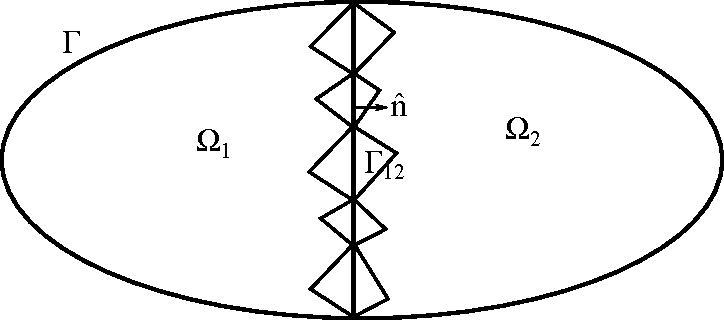
\includegraphics[width=12cm]{DDConforming}
\caption{Conforming domain decomposition sketch for two subdomains.}
\label{fig:DDConforming}
\end{figure}

Throughout this dissertation, the mesh is assumed to be conforming between adjacent domains, that is, all the elements at the boundaries are connected at their nodes as depicted in Fig. \ref{fig:DDConforming}. The choice of $\mathbf{v} = \hat{\mathbf{n}} \times \mathbf{w}$ has resulted, in terms of simplicity and convergence speed, the best choice. $\mathbf{v} = \hat{\mathbf{n}} \times \mathbf{w} \times \hat{\mathbf{n}}$ led to slower convergence in the iterative FETI-DP solution. The previous weak forms lead to the following systems
\begin{equation}
\label{eq:DDFETI1}
\begin{bmatrix}
A_{11} & A_{\Gamma_1 1} & \\
A_{\Gamma_1 1}^T & A_{\Gamma_1 \Gamma_1} & D_{11}\\
 & D_{11}^T  & T_{11}
\end{bmatrix}
\begin{bmatrix}
x_{1}\\
x_{\Gamma_1}\\
\lambda_{1}
\end{bmatrix}
=
\begin{bmatrix}
B_{1}\\
B_{\Gamma_1}\\
\phantom{x}
\end{bmatrix}
+
\begin{bmatrix}
\phantom{-}\phantom{A} & \phantom{-}\phantom{A} & \phantom{A}\\
\phantom{A} & \phantom{A} & \phantom{A}\\
\phantom{A} & D_{12}  & -T_{12}
\end{bmatrix}
\begin{bmatrix}
\phantom{A}\\
x_{\Gamma_2}\\
\lambda_{2}
\end{bmatrix},
\end{equation}
\noindent for the first subproblem and 
\begin{equation}
\label{eq:DDFETI2}
\begin{bmatrix}
A_{22} & A_{\Gamma_2 2} & \\
A_{\Gamma_2 2}^T & A_{\Gamma_2 \Gamma_2} & D_{22}\\
 & D_{22}^T  & T_{22}
\end{bmatrix}
\begin{bmatrix}
x_{2}\\
x_{\Gamma_2}\\
\lambda_{1}
\end{bmatrix}
=
\begin{bmatrix}
B_{2}\\
B_{\Gamma_2}\\
\phantom{x}
\end{bmatrix}
+
\begin{bmatrix}
\phantom{-}\phantom{A} & \phantom{-}\phantom{A} & \phantom{A}\\
\phantom{A} & \phantom{A} & \phantom{A}\\
\phantom{A} & D_{21}  & -T_{21}
\end{bmatrix}
\begin{bmatrix}
\phantom{x}\\
x_{\Gamma_1}\\
\lambda_{1}
\end{bmatrix},
\end{equation}
\noindent for the second one. The block matrices $\mat{A_{\Omega\Omega}}$, $\mat{A_{\Gamma_{\Omega}\Omega}}$ are $\mat{A_{\Gamma_{\Omega}\Gamma_{\Omega}}}$ those computed as in section \ref{sec:SchurDD}. The last block $\mat{D_{\Gamma\Gamma}}$ is the one that is retrieved by the coupling term integrals of \eqref{eq:j1} and \eqref{eq:j2}. The last row of block-matrices is retrieved by the testing of the transmission conditions \eqref{eq:RRTC} with the dual shape functions $\mathbf{v}$.
Explicitly, we have
\begin{gather*}
D_{mm} = k_0 \ \int_{\Gamma_{mn}} {\mathbf{v}_i^{m}}^* \cdot \hat{\mathbf{n}} \times\mathbf{w}_j^m \times \hat{\mathbf{n}} \ d\Gamma, \\
T_{mm} = jk_0 \ \int_{\Gamma_{mn}} {\mathbf{v}_i^{m}}^* \cdot \mathbf{v}_j^m \ d\Gamma,\\
D_{mn} = k_0 \ \int_{\Gamma_{mn}} {\mathbf{v}_i^{m}}^* \cdot \hat{\mathbf{n}} \times\mathbf{w}_j^n \times \hat{\mathbf{n}} \ d\Gamma, \\
T_{mn} = jk_0 \ \int_{\Gamma_{mn}} {\mathbf{v}_i^{m}}^* \cdot \mathbf{v}_j^n \ d\Gamma.
\end{gather*}
%
The systems of \eqref{eq:DDFETI1} and \eqref{eq:DDFETI2} can be solved directly in an alternating fashion within an iterative procedure. Starting from null solution vectors for each subdomain, $\mat{x}_1 = \mat{x_1 \ x_{\Gamma_1} \ \lambda_1}^T$ and $\mat{x}_2 = \mat{x_2 \ x_{\Gamma_2} \ \lambda_2}^T$, the procedure is expressed by the algorithm \ref{alg:FETIWISE}.
\begin{algorithm}[ht!]
\begin{algorithmic}
\caption{Domain-wise FETI-DP solution procedure.}
\label{alg:FETIWISE}
\State $\mat{x}_1^0 \gets 0$
\State $\mat{x}_2^0 \gets 0$
\State $k \gets 1$
\State $\mathit{err} \gets 1$
\While {$\mathit{err} \geq \mathit{maxerr}$}
    \State $\mat{x}_1^k \gets$ Solve \eqref{eq:DDFETI1}
    \State $\mat{x}_2^k \gets$ Solve \eqref{eq:DDFETI2}
    \State $\mathit{err} \gets \max \left(\frac{\Vert \mat{x}_1^k - \mat{x}_1^{k-1} \Vert}{\Vert \mat{x}_1^k\Vert}, \frac{\Vert \mat{x}_2^k - \mat{x}_2^{k-1} \Vert}{\Vert \mat{x}_2^k\Vert}\right)$ 
    \State $k \gets k+1$
\EndWhile
\end{algorithmic}
\end{algorithm}

One can also restrict the iterative procedure to the dual-primal unknowns. First a restriction matrix (boolean matrix) $\mat{R}_1$ is built as
$$ \mat{R}_1 = \begin{bmatrix}
\phantom{I_{P_1}} & I_{P_1} & \\
& & I_{D_1}
\end{bmatrix},$$
\noindent where $\mat{I_{P_1}}$ and $\mat{I_{D_1}}$ are unitary matrices of the size, respectively, of the number of primal and dual unknowns. Notice that the sizes might be different if $\Gamma_E$ crosses the boundary $\Gamma_{12}$. Than, the solution process is changed upon apply restriction to the subdomains solution vectors
%
\begin{multline}
\label{eq:DDFETI1res}
\begin{bmatrix}
x_{\Gamma_1}\\
\lambda_{1}
\end{bmatrix} =
\mat{R}_1
\begin{bmatrix}
x_{1}\\
x_{\Gamma_1}\\
\lambda_{1}
\end{bmatrix}
=\\
\mat{R}_1
\begin{bmatrix}
A_{11} & A_{\Gamma_1 1} & \\
A_{\Gamma_1 1}^T & A_{\Gamma_1 \Gamma_1} & D_{11}\\
 & D_{11}^T  & T_{11}
\end{bmatrix}^{-1}
\left(
\begin{bmatrix}
B_{1}\\
B_{\Gamma_1}\\
\phantom{x}
\end{bmatrix}
+
\begin{bmatrix}
\phantom{-}\phantom{A} & \phantom{-}\phantom{A} & \phantom{A}\\
\phantom{A} & \phantom{A} & \phantom{A}\\
\phantom{A} & D_{12}  & -T_{12}
\end{bmatrix}
\begin{bmatrix}
\phantom{x}\\
x_{\Gamma_2}\\
\lambda_{2}
\end{bmatrix}
\right) = \\
\underbrace{
\mat{R}_1
\begin{bmatrix}
A_{11} & A_{\Gamma_1 1} & \\
A_{\Gamma_1 1}^T & A_{\Gamma_1 \Gamma_1} & D_{11}\\
 & D_{11}^T  & T_{11}
\end{bmatrix}^{-1}
}_{(1)}
\left(
\begin{bmatrix}
B_{1}\\
B_{\Gamma_1}\\
\phantom{x}
\end{bmatrix}
+
\begin{bmatrix}
\phantom{A} & \phantom{A}\\
\phantom{A} & \phantom{A}\\
D_{12}  & -T_{12}
\end{bmatrix}
\begin{bmatrix}
x_{\Gamma_2}\\
\lambda_{2}
\end{bmatrix}
\right).
\end{multline}
\noindent Analogous matrices are computed for the second subproblem upon performing the changes in the subscripts $2 \rightarrow 1$ and $1 \rightarrow 2$. Notice that restriction matrices may result different for the second subproblem. The matrix factor $(1)$ lead to a small rectangular matrix (the row size is as the number of primal and dual unknowns on the boundaries) but dense due to matrix inversion. Once the procedure converged, the whole solution can be recovered by the solution of \eqref{eq:DDFETI1} and \eqref{eq:DDFETI2} where the dual and primal unknowns of the coarse problem provide the correct boundary conditions for continuity.

Several works \cite{Vouvakis2004,lee2005non,Vouvakis2006, li2006vector} have exploited the repetition of subdomains problems such as in finite periodic analyzes to considerably reduce the amount of matrices factors to compute. However, as we seek for the solution of arbitrarily shaped problems, the construction of many dense matrices may not be profitable. Hence, the path of constructing domain decomposition based preconditioners for Krylov subspace iterative solvers have been taken, as will be shown in the next sections. For this purpose, we formulate the global FETI-DP system to be solved with an iterative method as, collecting both systems \eqref{eq:DDFETI1} and \eqref{eq:DDFETI2} in a single global system,

\begin{equation}
\label{eq:FETIDPFull}
\begin{bmatrix}
A_{11} & A_{\Gamma_1 1} & & & & \\
A_{\Gamma_1 1}^T & A_{\Gamma_1 \Gamma_1} & D_{11} & & &\\
 & D_{11}^T  & T_{11} & \phantom{A} & -D_{12}  & T_{12}\\
& & & A_{22} & A_{\Gamma_2 2} &  \\
& & & A_{\Gamma_2 2}^T & A_{\Gamma_2 \Gamma_2} & D_{22}\\
\phantom{A} & -D_{21}  & T_{21} & & D_{22}^T  & T_{22}
\end{bmatrix}
\begin{bmatrix}
x_{1}\\
x_{\Gamma_1}\\
\lambda_{1}\\
x_{2}\\
x_{\Gamma_2}\\
\lambda_{2}
\end{bmatrix}
=
\begin{bmatrix}
\phantom{x}\\
B_{\Gamma_1}\\
\phantom{x}\\
\phantom{x}\\
B_{\Gamma_2}\\
\phantom{x}\\
\end{bmatrix}.
\end{equation}

\section[DD preconditioners for Krylov solvers]{Domain decomposition based preconditioners for Krylov subspace iterative solvers}

In this section, we present the Krylov subspace iterative solvers which exploit the optimality properties of projections (on Krylov spaces) during the iterative search process of the solution, with a deep control on the residual error (with error bounds) \cite{saad2000iterative}. In particular, we have employed the \textit{restarted-Generalized Minimum Residual} (GMRES($r$)) which finds the steepest descent upon applying projections in the residual norm between successive refinements of the solution. Its restarted approach is such that the basis vectors spanning the solution is restricted to a given number $r$, allowing to save memory requirements. Of course, the retarded version leads to different results respectively to the non-restarted version, as the whole projection bases are reset after $r$ iterations, and the next iteration cycle may start with a higher residual error.


\subsection{Restarted-Generalized Minimum Residual}

A general projection method for solving a linear system 
$$ \mat{A} \vect{x} = \vect{b}, $$ 
\noindent extracts an approximate solution $\vect{x}_m$ from an affine subspace $\vect{x}_0 + \mathcal{K}_m$ of dimension $m$ by imposing the Petrov-Galerkin condition
$$ \vect{b} - \mat{A}\vect{x}_m \perp \mathcal{L}_m$$
\noindent where $\mat{\mathcal{L}}_m$ is another subspace of dimension $m$. $\mat{x}_0$ is an initial guess to the solution.
A Krylov subspace method is such that
$$\mathcal{K}_m(\mat{A},\vect{r}_0) = \mathrm{span}\{\vect{r}_0, \mat{A}\vect{r}_0, \mat{A}^2\vect{r}_0,\ldots,\mat{A}^{m-1}\vect{r}_0\} $$
\noindent where $\vect{r}_0 = \vect{b}-\mat{A}\vect{x}_0$ is the residual. The vectors spanning $\mathcal{K}_m$ 
%(\mat{A},\vect{r}_0)$
might be almost linearly dependent. Thus, an appropriate orthonormalization is employed to build a Krylov subspace basis $\mat{V}_m = \mathrm{span}\left\{\vect{v}_1,\right.$ $\left.\ldots,\vect{v}_m 	\right\}$, the \textit{Arnoldi-Modified Gram-Schmidt} algorithm \ref{alg:Arnoldi}.
\begin{algorithm}[ht!]
\begin{algorithmic}
\caption{Arnoldi-Modified Gram-Schmidt.}
\label{alg:Arnoldi}
\State Choose a vector $\vect{v}_1$ such that $\Vert \vect{v}_1 \Vert_2 = 1$
\For {j = 1, \ldots, m}
    \State $\vect{w}_j \gets \mat{A} \vect{v}_j$
    \For {i = 1, \ldots, j}
    	\State $h_{i,j} \gets <\vect{w}_j,\vect{v}_i>$
		\State $\vect{w}_j \gets \vect{w}_j - h_{i,j} \vect{v}_i$
    \EndFor
    \State $h_{j+1,j} \gets \Vert \vect{w}_j \Vert_2$
    \If {$h_{j+1,j} = 0$} \State Break \EndIf
    \State $\vect{v}_{j+1} \gets \nicefrac{\vect{w}_j}{h_{j+1,j}} $
\EndFor
\end{algorithmic}
\end{algorithm}
%
\noindent The Arnoldi process produces and $\mathbb{R}^{m+1 \times m}$ upper Hessenberg matrix $\mat{H}_m$, coefficients for the expansion of $\mat{A}$ such that
\begin{eqnarray}
\label{eq:Hess}
\mat{A} \mat{V}_m &= &\mat{V}_{m+1} \mat{H}_m
\end{eqnarray}
\noindent Any vector $\vect{x} \in \vect{x}_0 + \mathcal{K}_m$ can be now written as
$$\vect{x} = \vect{x}_0 + \mat{V}_m \vect{y}$$
\noindent where $\vect{y}$ is a vector of dimension $m$. Defining 
$$J(\vect{y}) = \Vert \vect{b} - \mat{A} \vect{x} \Vert_2 = \Vert \vect{b} - \mat{A} (\vect{x}_0 + \mat{V}_m \vect{y})\Vert_2,$$
\noindent the relation \eqref{eq:Hess} results in
\begin{eqnarray*}
\vect{b} - \mat{A} \mat{V}_m &= &\vect{b} - {A}(\vect{x}_0 + \mat{V}_m \vect{y}),\\
&= & \vect{r}_0 - \mat{A} \mat{V}_m \vect{y},\\
&= & \beta\vect{v}_1 - \mat{V}_{m+1} \mat{H}_m \vect{y},\\
&= & \mat{V}_{m+1} \left( \beta\vect{e}_1 - \mat{H}_m \vect{y}\right).
\end{eqnarray*}
\noindent with $\beta = \Vert \vect{r}_0 \Vert_2$ and $\vect{v}_1 = \vect{r}_0/\beta$ is the first vector of unitary norm chose in the first step of the algorithm \ref{alg:Arnoldi}, and $\mat{V}_m^T\vect{r}_0 = \mat{V}_m^T(\beta\vect{v}_1) = \beta\vect{e}_1$ with $\vect{e}_1 = \vect{1 \ 0 \ \ldots \ 0}^T$ is the first standard basis vector. Since the column-vectors spanning $\mat{V}_{m+1}$ are orthonormal, then
$$J(\vect{y}) = \Vert \vect{b} - \mat{A} (\vect{x}_0 + \mat{V}_m \vect{y})\Vert_2 = \Vert \beta\vect{e}_1 - \mat{H}_m \vect{y} \Vert_2.$$
\noindent The GMRES \cite{saad1986gmres} (not yet restarted) approximation is the unique vector of $\vect{x}_0 + \mathcal{K}_m$  which minimizes $J(\vect{y})$. The approximation is obtained as $$\vect{x}_m = \vect{x}_0 + \mat{V}_m \vect{y}_m,$$ where $$\vect{y}_m = \mathrm{argmin}_y \Vert \beta\vect{e}_1 - \mat{H}_m \vect{y} \Vert_2.$$
%
\begin{algorithm}[ht!]
\begin{algorithmic}
\caption{Restarted-Generalized Minimum Residual.}
\label{alg:rGMRES}
\While {$\beta = \Vert \vect{r}_0 \Vert_2 \geq \mathit{maxerr}$  with $\vect{r}_0 = \vect{b} - {A}(\vect{x}_0$, $\vect{v}_1 = \vect{r}_0/\beta$}
	\For {$m = 1,\ldots, r$}
	\State Generate the Arnoldi basis and $\mat{H}_m$
	\State Compute $\vect{y}_m$ which minimizes $\Vert \beta\vect{e}_1 - \mat{H}_m \vect{y} \Vert_2$ 
	\State Compute $\vect{x}_m = \vect{x}_0 + \mat{V}_m \vect{y}_m$
	\EndFor
	\State $\vect{x}_0 \gets \vect{x}_m$ \Comment{The new starting vector is $\vect{x}_m$}
\EndWhile
\end{algorithmic}
\end{algorithm}
%
%An important result on the convergence of symmetric positive definite matrices (as those analyzed ) is that
%$$\Vert \vect{r}_n \Vert_2 \leq \left(\frac{2 \mathsf{k}_2(\mat{A})-1}{2 \mathsf{k}_2(\mat{A})}\right)^{{n}/{2}} \Vert \vect{r}_0 \Vert_2$$
%\noindent where $\mathsf{k}_2(\mat{A})$ is the condition number of the system matrix.

A well known difficulty with the restarted GMRES algorithm is that it can stagnate
when the matrix is not positive-definite\footnote{Certain boundary conditions (especially for radiation and waveports continuity) and  materials properties may lead to non-positive-definite system matrices.}. The full GMRES algorithm is guaranteed to converge in at most $N$ steps ($N$ the system dimensions), but this would be impractical if there were many steps required for convergence, due to large memory requirements: $O(N^2)$, similar to sparse direct solvers, whereas the restarted has only $O(rN)$ memory requirements. 

A typical remedy is to use preconditioning techniques whose goal is to reduce the number of steps required to converge. Here follow two types of preconditioners: the block Jacobi and the block Gauss-Seidel. None of these involve the computation of a Schur complement matrix, as a direct assembly of this matrix and its inversion without proper approximation may lead, for very large problem, to memory bottlenecks.

\subsection{Block Jacobi preconditioner}\label{sec:JC}

Let us consider the linear system of equations that leads to the following matrix system 
\begin{equation}
\label{eq:SysBlocks}
\begin{bmatrix}
A_{11} & A_{12} & A_{13}\\
A_{21} & A_{22} & A_{23}\\
A_{31} & A_{32} & A_{33}
\end{bmatrix}
\begin{bmatrix}
x_{1}\\
x_{2}\\
x_{3}
\end{bmatrix}
=
\begin{bmatrix}
b_{1}\\
b_{2}\\
b_{3}
\end{bmatrix},
\end{equation}
\noindent where $\mat{A}$ is non necessarily symmetric and we have considered only a single right-hand side vector as the GMRES($r$) solves for one right-hand side at a time. The block Jacobi preconditioner is defined as
\begin{equation}
\label{eq:jc}
\mat{P}_{J}
=
\begin{bmatrix}
A_{11} &  & \\
 & A_{22} & \\
 & & A_{33}
\end{bmatrix},
\end{equation}
\noindent and the resulting preconditionned system is
\begin{multline}
\begin{bmatrix}
\mat{A_{11}}^{-1} &  & \\
 & \mat{A_{22}}^{-1} & \\
 & & \mat{A_{33}}^{-1}
\end{bmatrix}
\begin{bmatrix}
A_{11} & A_{12} & A_{13}\\
A_{21} & A_{22} & A_{23}\\
A_{31} & A_{32} & A_{33}
\end{bmatrix}
\begin{bmatrix}
x_{1}\\
x_{2}\\
x_{3}
\end{bmatrix}
=\\
\begin{bmatrix}
\mat{A_{11}}^{-1} &  & \\
 & \mat{A_{22}}^{-1} & \\
 & & \mat{A_{33}}^{-1}
\end{bmatrix}
\begin{bmatrix}
b_{1}\\
b_{2}\\
b_{3}
\end{bmatrix},
\end{multline}
\noindent where we have exploited the following relation on the inversion of block diagonal matrices
$$ 
\begin{bmatrix}
A_{11} &  & \\
 & A_{22} & \\
 & & A_{33}
\end{bmatrix}^{-1} = 
\begin{bmatrix}
\mat{A_{11}}^{-1} &  & \\
 & \mat{A_{22}}^{-1} & \\
 & & \mat{A_{33}}^{-1}
\end{bmatrix}.
$$
\noindent Preconditioning with $\mat{P}_{J}$ is integrated in the GMRES($r$) algorithm after the computation of the residual vector $\vect{r}_m = \vect{b} - \mat{A} (\vect{x}_0 + \mat{V}_m \vect{y}) = \vect{\vect{r_1}_m \ \vect{r_2}_m \ \vect{r_3}_m}^T$ upon performing
\begin{eqnarray*}
\vect{r_1}_m &\longleftarrow & \mat{A_{11}}^{-1}\vect{r_1}_m, \\
\vect{r_2}_m &\longleftarrow & \mat{A_{22}}^{-1}\vect{r_2}_m, \\
\vect{r_3}_m &\longleftarrow & \mat{A_{33}}^{-1}\vect{r_3}_m. 
\end{eqnarray*}

\subsection{Block Gauss-Seidel preconditioner} \label{sec:GS}

Let us consider again the matrix system \eqref{eq:SysBlocks}, the lower block Gauss-Seidel preconditioner is defined as
\begin{equation}
\label{eq:gs}
\mat{P}_{GS}
=
\begin{bmatrix}
A_{11} &  & \\
A_{21} & A_{22} & \\
A_{31} & A_{32} & A_{33}
\end{bmatrix}.
\end{equation}
\noindent The inversion of the whole $\mat{P}_{GS}$ results, in the case of symmetric Schur complement based domain decomposition, to the solution of the problem, hence at the cost of a direct solver. In any case, the computational requirements may be prohibitive for large problems. However, it can be shown that the inverse of $\mat{P}_{GS}$
\begin{gather}
\begin{bmatrix}
A_{11} &  & \\
A_{21} & A_{22} & \\
A_{31} & A_{32} & A_{33}
\end{bmatrix}^{-1} = 
\begin{bmatrix}
\mat{A_{11}}^{-1} &  & \\
\tilde{\mat{A_{21}}} & \mat{A_{22}}^{-1} & \\
\tilde{\mat{A_{31}}} & \tilde{\mat{A_{32}}} & \mat{A_{33}}^{-1}
\end{bmatrix},
\end{gather}
\noindent where
\begin{eqnarray*}
\tilde{\mat{A_{21}}} &= &-\mat{A_{22}}^{-1}\mat{A_{21}}\mat{A_{11}}^{-1},\\
\tilde{\mat{A_{32}}} &= &-\mat{A_{33}}^{-1} \mat{A_{32}} \mat{A_{22}}^{-1},\\
\tilde{\mat{A_{31}}} &= &\mat{A_{33}}^{-1}\mat{A_{32}}\mat{A_{22}}^{-1}\mat{A_{21}}\mat{A_{11}}^{-1}- \mat{A_{33}}^{-1}\mat{A_{31}}\mat{A_{11}}^{-1},
\end{eqnarray*}
\noindent can be computed sequentially on the residual vector, updating it progressively while computing the diagonal blocks inverse. Preconditioning with $\mat{P}_{GS}$ is integrated in the GMRES($r$) algorithm after the computation of the residual vector $\vect{r}_m = \vect{b} - \mat{A} (\vect{x}_0 + \mat{V}_m \vect{y}) = \vect{\vect{r_1}_m \ \vect{r_2}_m \ \vect{r_3}_m}^T$ upon performing sequentially
\begin{eqnarray*}
\vect{r_1}_m &\longleftarrow & \mat{A_{11}}^{-1}\vect{r_1}_m, \\
\vect{r_2}_m &\longleftarrow & \mat{A_{22}}^{-1}\left(\vect{r_2}_m - \mat{A_{21}} \vect{r_1}_m \right).\\
\vect{r_3}_m &\longleftarrow & \mat{A_{33}}^{-1}\left(\vect{r_3}_m - \mat{A_{31}} \vect{r_1}_m - \mat{A_{32}} \vect{r_2}_m\right).\\
\end{eqnarray*}


\section{Numerical tests}

In this section, we present several results on a simple test case, that of a WR-90 rectangular waveguide segment, where the mesh is partitioned in order to implement the domain decomposition formulations. First, a simple two-domains test will be performed to assess the methods without iterative solvers. Then, the performances of the preconditioners will be analyzed, also varying the number of subdomains. %Finally, the analysis of a FSS-radome enclosed patch antennas array will be tackled.

\subsection{WR-90 rectangular waveguide}

The model analyzed consists of a 240~mm long $\hat{\mathbf{x}}$-directed WR-90 waveguide segment. The metallic walls are considered perfect electric conductors  while the two waveports are located at the extremities in the $\hat{\mathbf{x}}$ direction. The mesh consists of 20,602 tetrahedra and has been partitioned, using Metis \cite{karypis1995metis}, into two parts separated by an arbitrarily shaped surface composed by faces shared by tetrahedra located in the middle of the segment. Actually, Metis divides a mesh such that the parts result to have approximately the same number of tetrahedra (10,489 and 10,113).

\begin{figure}[h!]
\centering
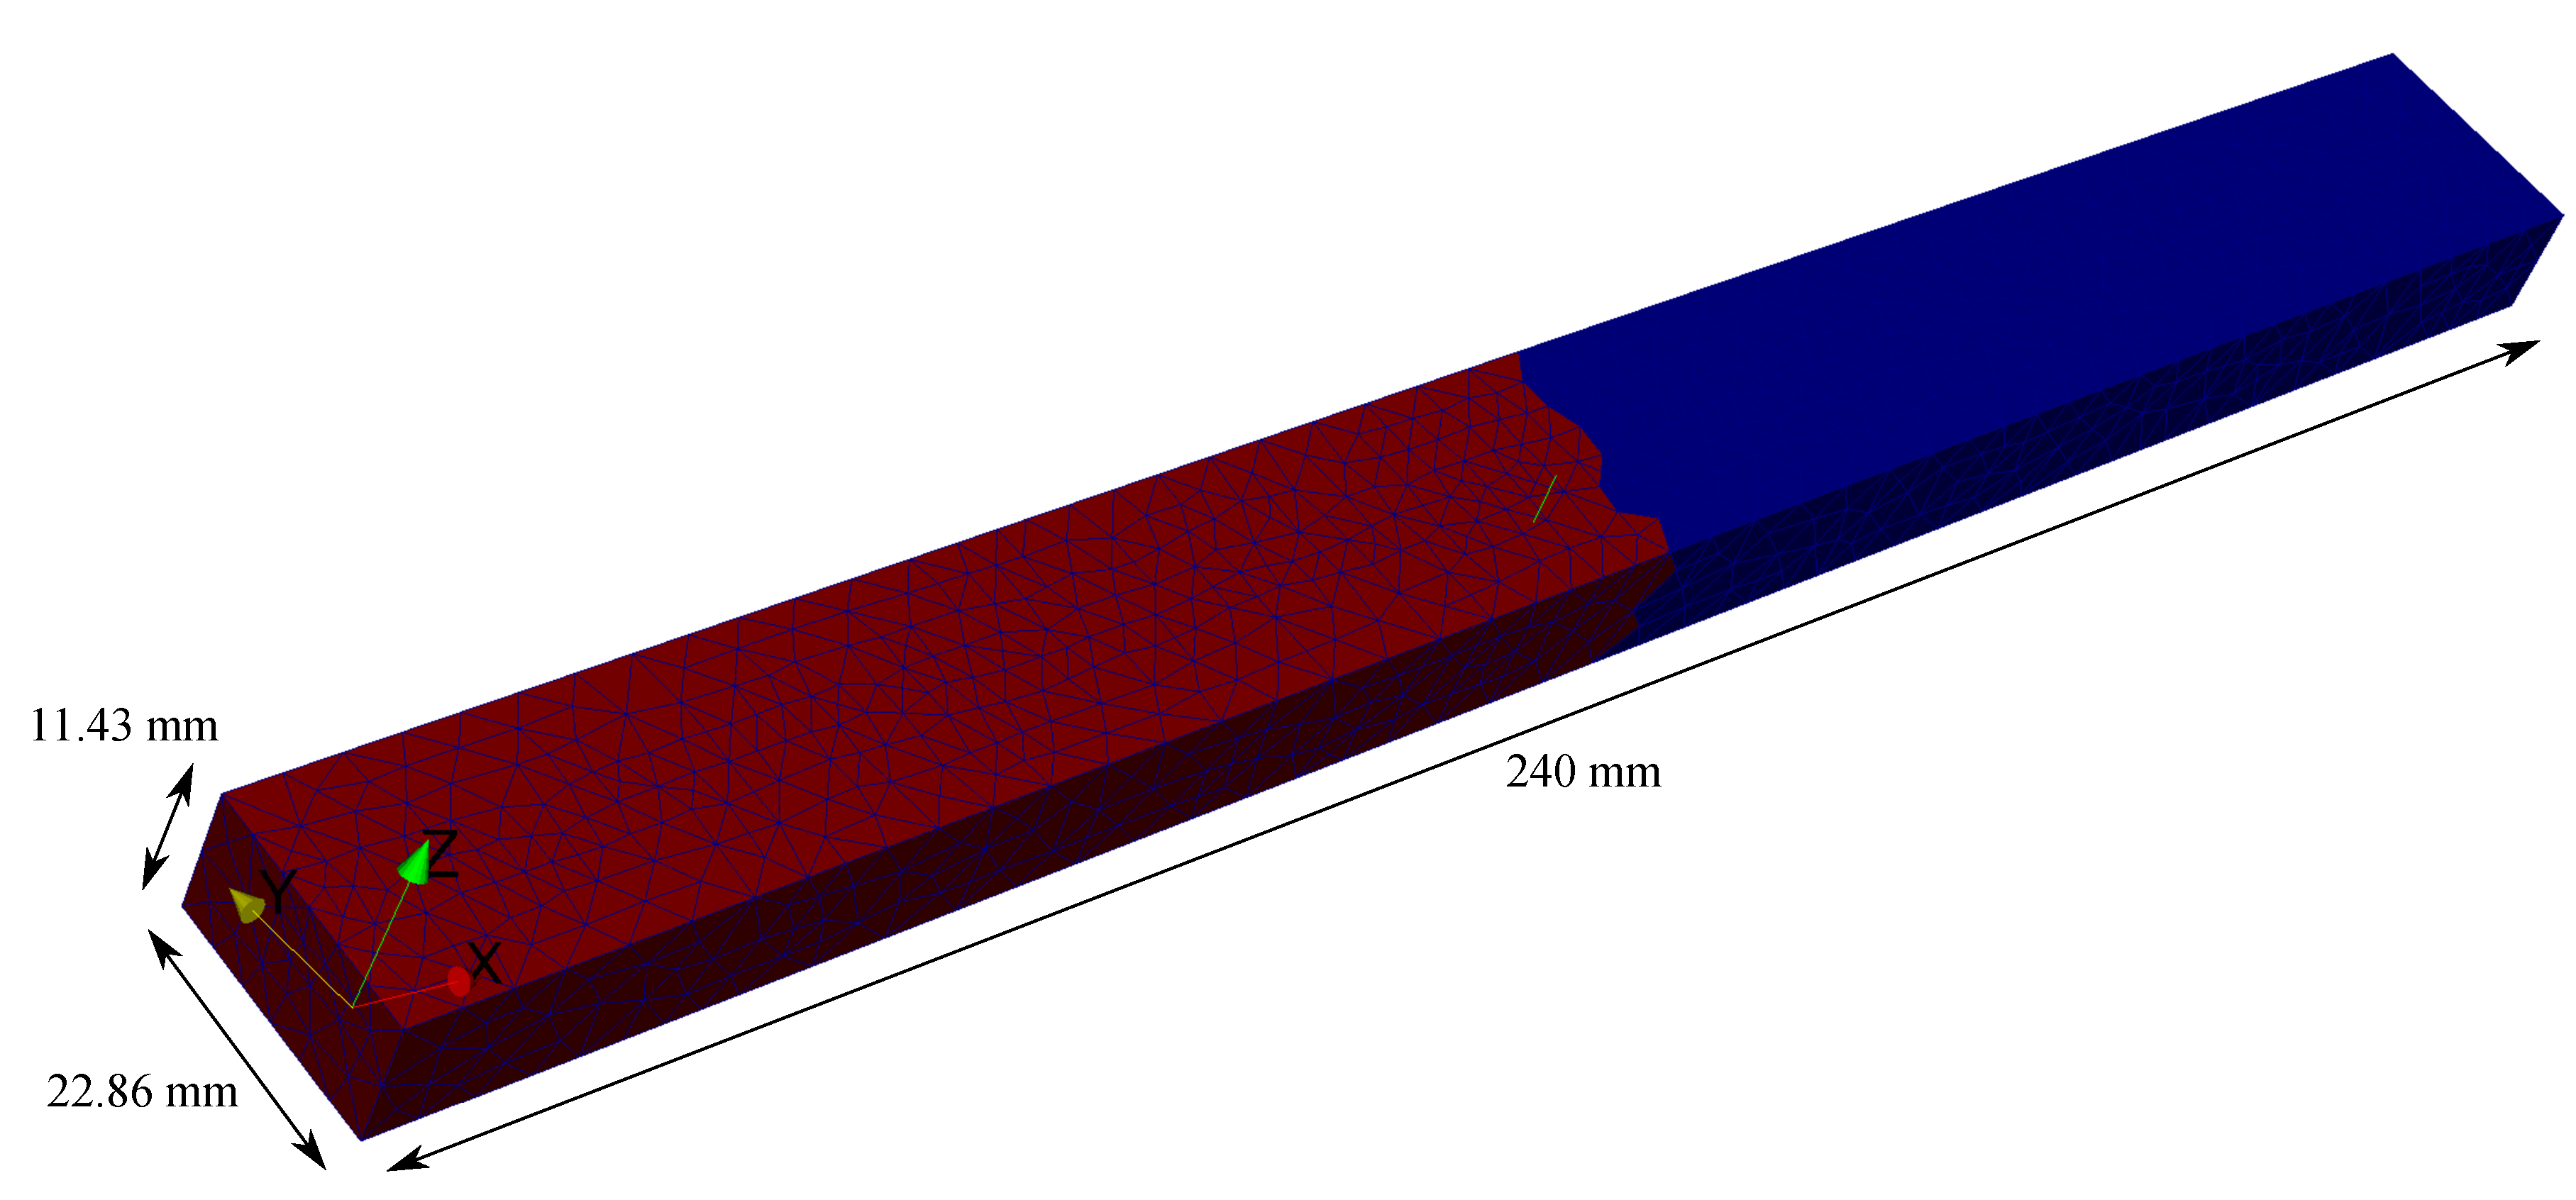
\includegraphics[width=\textwidth]{WR90Part}
\caption{$\hat{\mathbf{x}}$-directed WR-90 waveguide segment and conformal mesh partitioning.}
\label{fig:WR90Part}
\end{figure}

\subsection{Direct analysis}

The first conducted analysis is a direct solution of the whole problem upon imposing either dominant mode (DOM) or transfinite element method (TFE) on the waveports, and computing its spectral response over the mono-modal bandwidth. First order basis functions have been used to compute the scattering parameters ($\mathrm{TE}_{10}$) of Fig. \ref{fig:WRfreq}.

\begin{figure}[h!]
\centering
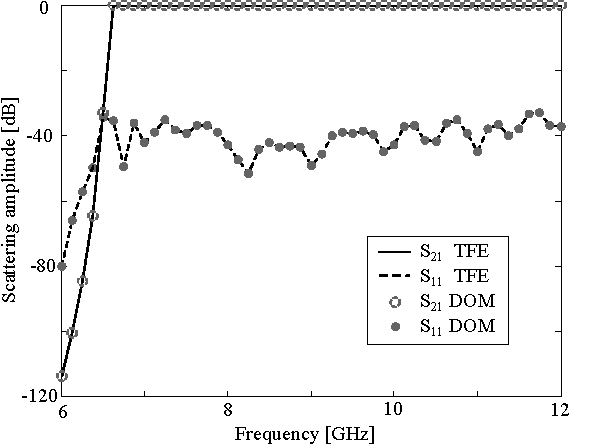
\includegraphics[width=13.4cm]{WRfreq}
\caption{Frequency response of the WR-90 waveguide segment.}
\label{fig:WRfreq}
\end{figure}

As expected, all the power is transmitted to the second port only when the frequency of excitation is higher than the cut-off frequency of 6.557 GHz for the $\mathrm{TE}_{10}$ mode in a WR-90. No significant differences are noticed between TFE and DOM for this frequency range. The peak memory required by the process was of about 50~MB and the times for assembly and solve of 0.7~s for each frequency point.

\subsection{Schur complement analysis}

Next, the Schur complement solution is performed. The assembled DD system matrix is shown in Fig. \ref{fig:DDSchurMat}. The assembly timings were of about 2.5~s. While the direct solution required only 0.45~s, the Schur approach required considerably more times and memory, as reported in table \ref{tab:SchurSol}. The assembly of the Schur complement matrix required approximately 10~s, due principally to the 155 column vectors of $\mat{A_{\Gamma 1}}^T$ which have to be multiplied by the dense matrix $\mat{A_{11}}^{-1}$. This step can be enhanced, exploiting the fact many of these column vectors are identically null. The computation of boundary unknowns is rather rapid and inexpensive for their small dimensions. The high density of the Schur complement matrix is shown in Fig. \ref{fig:DDSchurMatS}. Even if symmetries are exploited, the use of direct solvers ($O(N^3)$) would quickly lead to memory overload. The scattering parameters computed by this solution are reported in Fig. \ref{fig:WRfreqSchur} , as the maximum error recorded in this process has been of $\approx 10^{-12}$ in both TFE and DOM excitations.

\begin{table}[ht!]
\begin{center}
\begin{tabular}{|c|c|c|}
\hline 
Step & Time & Memory \\ 
\hline
\hline 
$\mat{A_{\Gamma 1}} \mat{A_{11}}^{-1} \mat{A_{\Gamma 1}}^T$ (8557) & 5.2~s & 10~MB\\ \hline 
$\mat{A_{\Gamma 2}} \mat{A_{22}}^{-1} \mat{A_{\Gamma 2}}^T$ (8082) & 4.8~s & 9.5~MB\\ \hline 
$\mat{x_\Gamma} = \mat{S}^{-1} \mat{G}$ (155) & 0.002~s & < 1~MB\\ \hline 
$\mat{x_1} = \mat{A_{11}}^{-1} (-\mat{A_{\Gamma 1}}^T \mat{x_\Gamma})$ & 0.15~s &  2~MB\\ \hline 
$\mat{x_2} = \mat{A_{22}}^{-1} (-\mat{A_{\Gamma 2}}^T \mat{x_\Gamma})$ & 0.14~s &  2~MB\\ \hline 
\end{tabular}
\end{center}
\caption{Direct Schur solution times and memory requirements.}
\label{tab:SchurSol}
\end{table}

\begin{figure}[ht!]
\centering
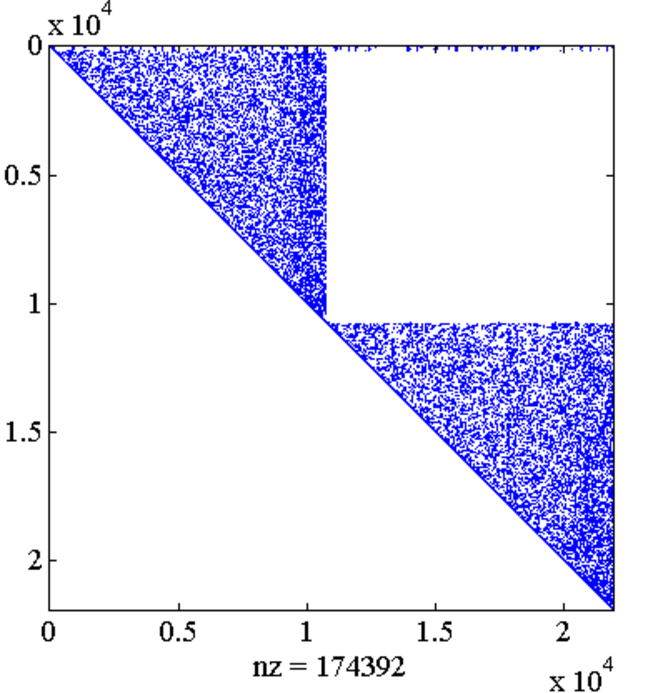
\includegraphics[width=12cm]{DDSchurMat}
\caption{Upper triangular part of the Schur complement based domain decomposition system matrix.}
\label{fig:DDSchurMat}
\end{figure}

\begin{figure}[ht!]
\centering
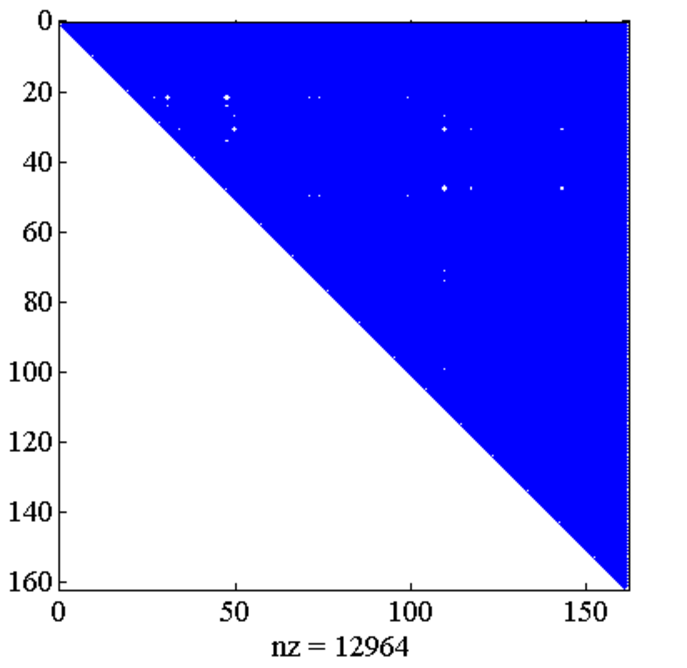
\includegraphics[width=8cm]{DDSchurMatS}
\caption{Upper triangular part of the Schur complement matrix.}
\label{fig:DDSchurMatS}
\end{figure}

\begin{figure}[ht!]
\centering
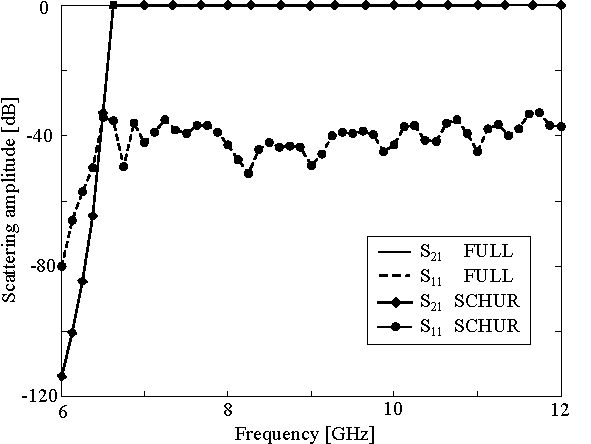
\includegraphics[width=13.4cm]{WRfreqSchur}
\caption{Frequency response of the WR-90 waveguide segment computed with the Schur complement algorithm.}
\label{fig:WRfreqSchur}
\end{figure}

\clearpage
\subsubsection{FETI-DP analysis}

We proceed with the analysis employing the FETI-DP algorithm in his version restricted to dual-primal unknowns. The global matrix, assembled as a whole for Fig. \ref{fig:DDFETIMat}, is composed of a block-diagonal part which is symmetric and and non-symmetric off-diagonal blocks parts.

\begin{figure}[ht!]
\centering
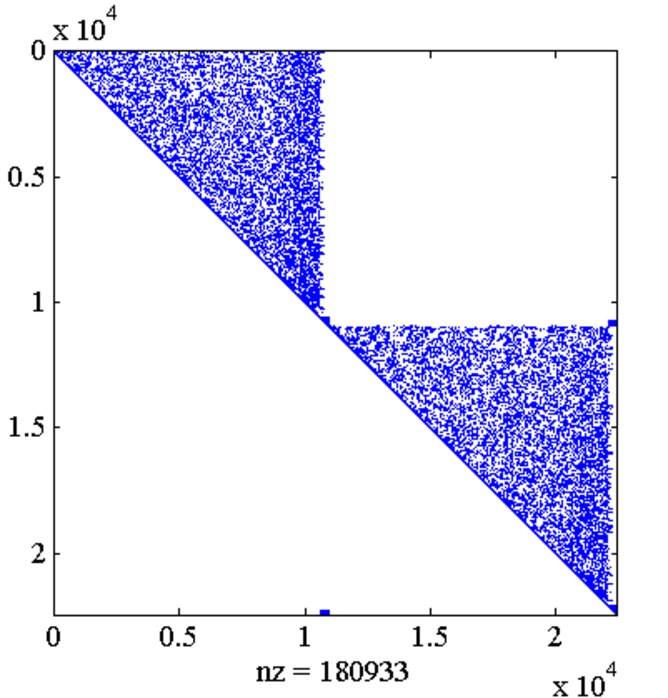
\includegraphics[width=12cm]{DDFETIMat}
\caption{FETI-DP based domain decomposition global system matrix. The upper triangular part of the symmetric blocks are  shown to enhance visibility of these parts. }
\label{fig:DDFETIMat}
\end{figure}

The first test is performed exciting the structure with DOM at 10~GHz. The convergence history in the relative error between successive approximations of the dual-primal unknowns on the boundary is shown in Fig. \ref{fig:Convergence}. The algorithm required in the average 430 iterations ($\approx 200~\mathrm{s}$) to achieve an error of $10^{-2}$. The spectral response, when dominant mode boundary condition on waveports is used, is depicted in Fig. \ref{fig:WRfreqFETI}. An average Euclidean error on the spectrum is of 2.1~\%.

The poor convergence behavior is due to a non-optimal residual minimization. This result has motivated the use of the FETI-DP as a preconditioner for Krylov iterative solvers which not only guarantee the convergence of the solution, but somehow choose the best directions.


\begin{figure}[ht!]
\centering
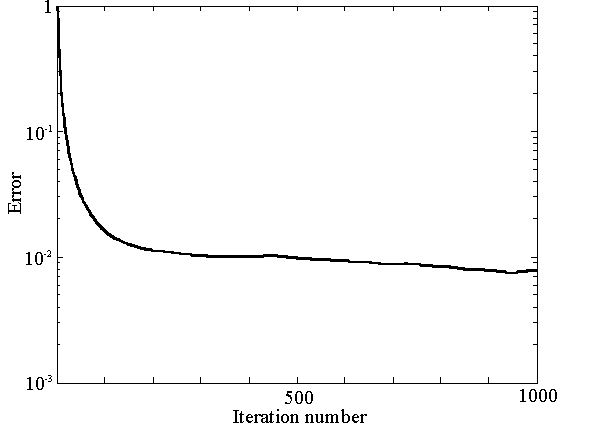
\includegraphics[width=13.4cm]{Convergence}
\caption{Convergence history of the restricted FETI-DP algorithm.}
\label{fig:Convergence}
\end{figure}

\begin{figure}[h!]
\centering
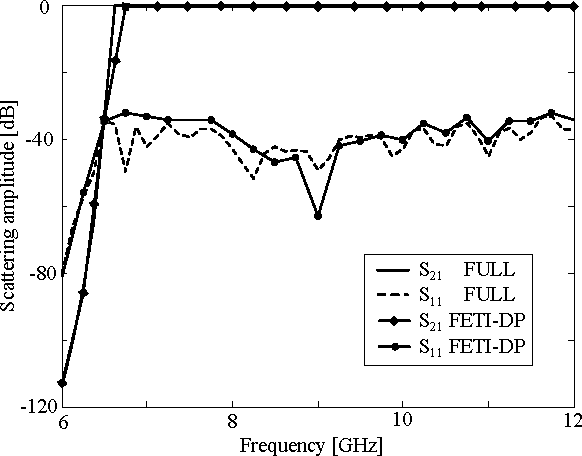
\includegraphics[width=13.4cm]{WRfreqFETI}
\caption{Comparison of the frequency response computed with direct full-domain solution and restricted FETI-DP (dominant mode waveports).}
\label{fig:WRfreqFETI}
\end{figure}
\clearpage

\subsection{\texorpdfstring{DD preconditioned GMRES($r$)}{DD preconditioned GMRES(r)}}

One of the main advantage of iterative solvers, when convergence is guaranteed, is the possibility to achieve approximate solutions within a prescribe tolerance. In many practical applications, the gaps between the CAD model, virtual, and the realized model are such that their electromagnetic behaviors differ of some \quotes{realization tolerances}. Hence, it may not be necessary to achieve numerical precision for acceptable simulation results. The numerical solution tolerance may be limited to one or a couple of magnitude orders lower to keep relatively good agreement with the real model.

Direct solvers might be used in single precision to decrease computational resources demand, but they still suffer from quadratic complexity for sparse matrices. One may also use an iterative solver, limiting the residual (error) norm to the desired tolerance. However the convergence speed, and hence the number of iterations and the overall computational times, tightly depend on the conditioning of the system matrix. It is also known that the conditioning gets worse as the problem gets larger. Adequate preconditioning of large problems matrices has to be performed in order to tackle iterative solutions in relatively acceptable amount of times. We will see that, due to block-matrix form of the domain decomposition systems, one can compute almost inexpensive very good preconditioners to tackle large problems.

\subsubsection{Performances of the various preconditioners}

To compare the performances of preconditioners, the WR-90 waveguide segment, partitioned in two subdomains as in Fig. \ref{fig:WR90Part}, have been analyzed at 10~GHz using double precision direct solvers to invert block-diagonal matrices. The results are compared with non-preconditioned full-domain solution. A restarting size of $r=100$ has been chosen and the residual error set to $10^{-12}$. 

\begin{figure}[h!]
\centering
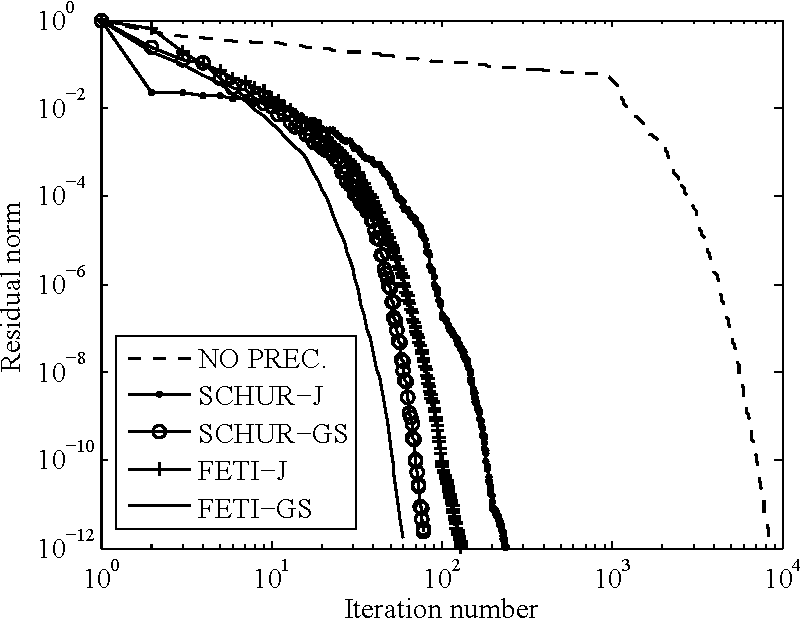
\includegraphics[width=13.4cm]{GMREScomp}
\caption{Comparison between the domain decomposition preconditioners and not preconditioned full-domain GMRES(100) solution.}
\label{fig:GMREScomp}
\end{figure}

Due to low residual error, all the simulation converge to the accuracy of a double precision sparse direct solution. This demonstrates that even the global FETI-DP problem is well posed and no energy is lost within interconnecting process (with only one interface). The effect of the restarting after 100 iterations can be appreciated on the DD-SCHUR Jacobi preconditioner run. In fact, after 100 and 200 iterations, the descent of the residual norm varies, leading for some iterations to a slower convergence.

\begin{table}[h!]
\begin{center}
\begin{tabular}{|c|c|c|c|}
\hline 
Solver & Iterations & Time & Peak memory \\ 
\hline
\hline 
Direct (double precision) & - & 1~s & 49.5~MB\\ \hline 
No preconditioner & 8459 & 276~s & 68.2~MB\\ \hline 
DD-Schur Jacobi precond. & 238 & 160~s & 68.6~MB\\ \hline 
DD-Schur Gauss-Seidel precond. & 78 & 54.5~s & 69.1~MB\\ \hline 
DD-FETI Jacobi precond. & 130 & 90~s & 69.7~MB\\ \hline 
DD-FETI Gauss-Seidel precond. & 58 & 41.8~s & 69.2~MB\\ \hline 
\end{tabular}
\end{center}
\caption{Times and memory requirements for different GMRES(100) runs at 10~GHz.}
\label{tab:gmresComp}
\end{table}

While the full-domain non preconditioned solution required about 276~s (8459 iterations), the domain decomposition preconditioners allowed to reduce the amount of times as shown in table \ref{tab:gmresComp}. The memory required by all the runs has been of about 69~MB, mainly allocated for the 100 orthonormal vectors (dense) used as Krylov space basis. In fact, all the assembled matrices required approximately 24~MB and the mesh about 10~MB.

It is clear that the Gauss-Seidel preconditioner leads to a better conditioning of the system matrix in both DD-SCHUR and DD-FETI cases. Let us analyze the performances of these solvers as the frequency of excitation varies (8, 10 and 12~GHz).

\begin{figure}[h!]
\centering
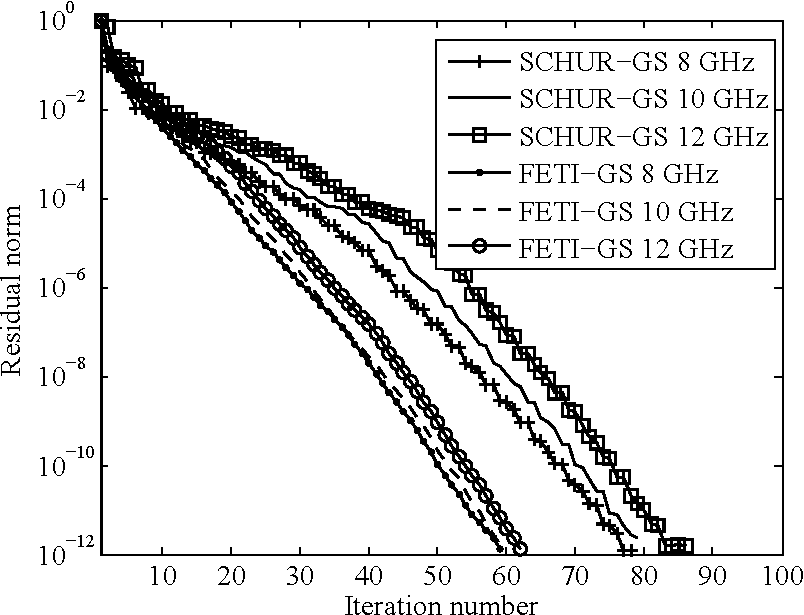
\includegraphics[width=13.4cm]{DDfreqComp}
\caption{Comparison between the SCHUR and FETI Gauss-Seidel preconditioned GMRES(100) runs as the frequency of excitation varies.}
\label{fig:DDfreqComp}
\end{figure}

As expected \cite{dyczij1999efficient}, the condition number of the system matrices grows with the frequency, resulting in more iterations (Fig. \ref{fig:DDfreqComp}). The FETI approach behaves clearly better that the SCHUR alternative. However, the SCHUR approach remains an invaluable method for arbitrary domain partitioning, as the transfinite element waveports boundary conditions (with better accuracy) can be straightforwardly implemented. In fact, waveports interfaces shared by multiple subdomains may lead to non strictly block-diagonal system matrices and hence worse performances.

\begin{figure}[h!]
\centering
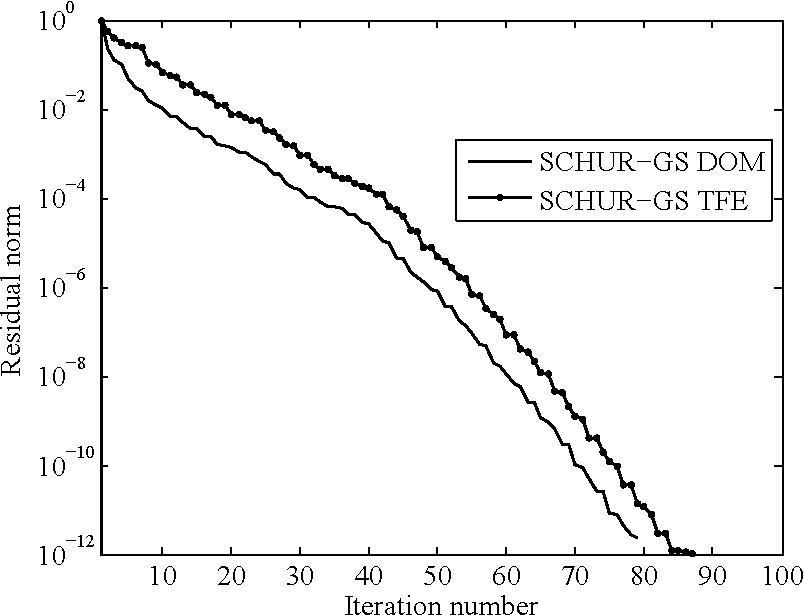
\includegraphics[width=13.4cm]{schurdomtfe}
\caption{Convergence history for SCHUR-GS GMRES(100) solution at 10~GHz with either dominant mode or transfinite element method waveports boundary conditions.}
\label{fig:schurdomtfe}
\end{figure}

In Fig. \ref{fig:schurdomtfe}, the convergence of both dominant mode and transfinite element waveports are shown. The higher accuracy of mode continuity is paid with a worse conditioning of the global DD-SCHUR system matrix.

As we are typically interested in error controlled solvers, we proceed evaluating the error induced in the scattering parameters while varying the maximum residual error. Several runs have been performed, considering dominant mode waveports boundary conditions at 10~GHz. Table \ref{tab:Sacc} shows that the FETI based method achieves faster a better overall accuracy than the Schur complement based. Also, while the scattering parameters error in the Schur complement based method might not be strictly lower than the prescribed residual error, in the case of the FETI they are.
However, when employing the transfinite element method on the waveports, the Schur complement based method behaves differently as shown in table \ref{tab:SaccTFE}, assuring an error lower than the prescribed residual error. 

\begin{sidewaystable}[h]
\begin{center}
\begin{tabular}{|c|c|c|c|c|}
\hline 
Solver & Residual error & $|S_{11}|$~[dB] & $|S_{21}|$~[dB] & $\frac{\Vert |S_\mathrm{ref}| - |S| \Vert_{2}}{\Vert|S_\mathrm{ref}|\Vert_2}$\\ 
\hline
\hline 
Direct (reference) & - & -42.8389 & -0.0024 & 0\\ \hline \hline
\setlength{\arrayrulewidth}{0.5pt}
DD-Schur Gauss-Seidel preconditioned & $10^{-2}$ & -26.7529 & -0.1958 & $2.23~10^{-2}$\\ \hline 
"& $10^{-4}$ & -42.5118 & -0.0030 & $1.4234~10^{-4}$\\ \hline 
"& $10^{-6}$ & -42.8397 & -0.0025 & $4.0786~10^{-7}$\\ \hline 
"& $10^{-8}$ & -42.8389 & -0.0024 & $3.4517~10^{-9}$\\ \hline 
"& $10^{-10}$ & -42.8389 & -0.0024 & $8.2561~10^{-11}$\\ \hline
"& $10^{-12}$ & -42.8389 & -0.0024 & $1.2571~10^{-13}$\\ \hline \hline
DD-FETI Gauss-Seidel preconditioned & $10^{-2}$ & -40.5331 & -0.0603 & $3.5~10^{-3}$\\ \hline 
"& $10^{-4}$ & -42.8404 & -0.0024 & $2.0280~10^{-6}$\\ \hline 
"& $10^{-6}$ & -42.8389 & -0.0024 & $1.1615~10^{-8}$\\ \hline 
"& $10^{-8}$ & -42.8389 & -0.0024 &  $5.5698~10^{-10}$\\ \hline 
"& $10^{-10}$ & -42.8389 & -0.0024 & $1.8771~10^{-12}$\\ \hline
"& $10^{-12}$ & -42.8389 & -0.0024 & $1.7357~10^{-14}$\\ \hline
\end{tabular}
\end{center}
\caption{Scattering parameters accuracy for different prescribed residual errors (runs at 10~GHz with dominant mode on waveports).}
\label{tab:Sacc}
\end{sidewaystable}

\begin{sidewaystable}[h]
\begin{center}
\begin{tabular}{|c|c|c|c|c|}
\hline 
Solver & Residual error & $|S_{11}|$~[dB] & $|S_{21}|$~[dB] & $\frac{\Vert |S_\mathrm{ref}| - |S| \Vert_{2}}{\Vert|S_\mathrm{ref}|\Vert_2}$\\ 
\hline
\hline 
Direct (reference) & - & -42.8035  & -0.0002 & 0\\ \hline \hline
\setlength{\arrayrulewidth}{0.5pt}
DD-Schur Gauss-Seidel preconditioned& $10^{-2}$ & -35.1814  & -0.0682 & $6.4~10^{-3}$\\ \hline 
"& $10^{-4}$ & -42.7897 &  -0.0002 & $6.8925~10^{-6}$\\ \hline 
"& $10^{-6}$ & -42.8034 &  -0.0002 & $1.3365~10^{-7}$\\ \hline 
"& $10^{-8}$ & -42.8035 &  -0.0002 & $3.9561~10^{-10}$\\ \hline
"& $10^{-10}$ & -42.8035 &  -0.0002 & $8.2355~10^{-12}$\\ \hline
"& $10^{-12}$ & -42.8035 &  -0.0002 & $2.0021~10^{-13}$\\ \hline
\end{tabular}
\end{center}
\caption{Scattering parameters accuracy for different prescribed residual errors (runs at 10~GHz with transfinite elements on waveports).}
\label{tab:SaccTFE}
\end{sidewaystable}

In the case of simply partitioned electromagnetic devices, the use of SCHUR-TFE (simply SCHUR) and FETI-DOM (simply FETI) might result to be reliable in the sense of the residual error. The first usually requires more iterations than the second (hence more time), but as it results from the formulation, should provide more accurate results, especially in multi-mode analyzes in which higher-order modes are excited.

\clearpage
\subsubsection{Performances against subdomains number}

We proceed analyzing the behavior of both SCHUR and FETI (with Gauss-Seidel preconditioners) while increasing the number of domains on the same mesh. A residual error of $10^{-4}$ can be retained, as it leads in both cases to a very good approximation of the solution. The whole waveguide is partitioned using Metis in 4, 8, 12 and 16 subdomains as depicted in Fig. \ref{fig:Partitions}. 

\begin{figure}[h!]
\centering
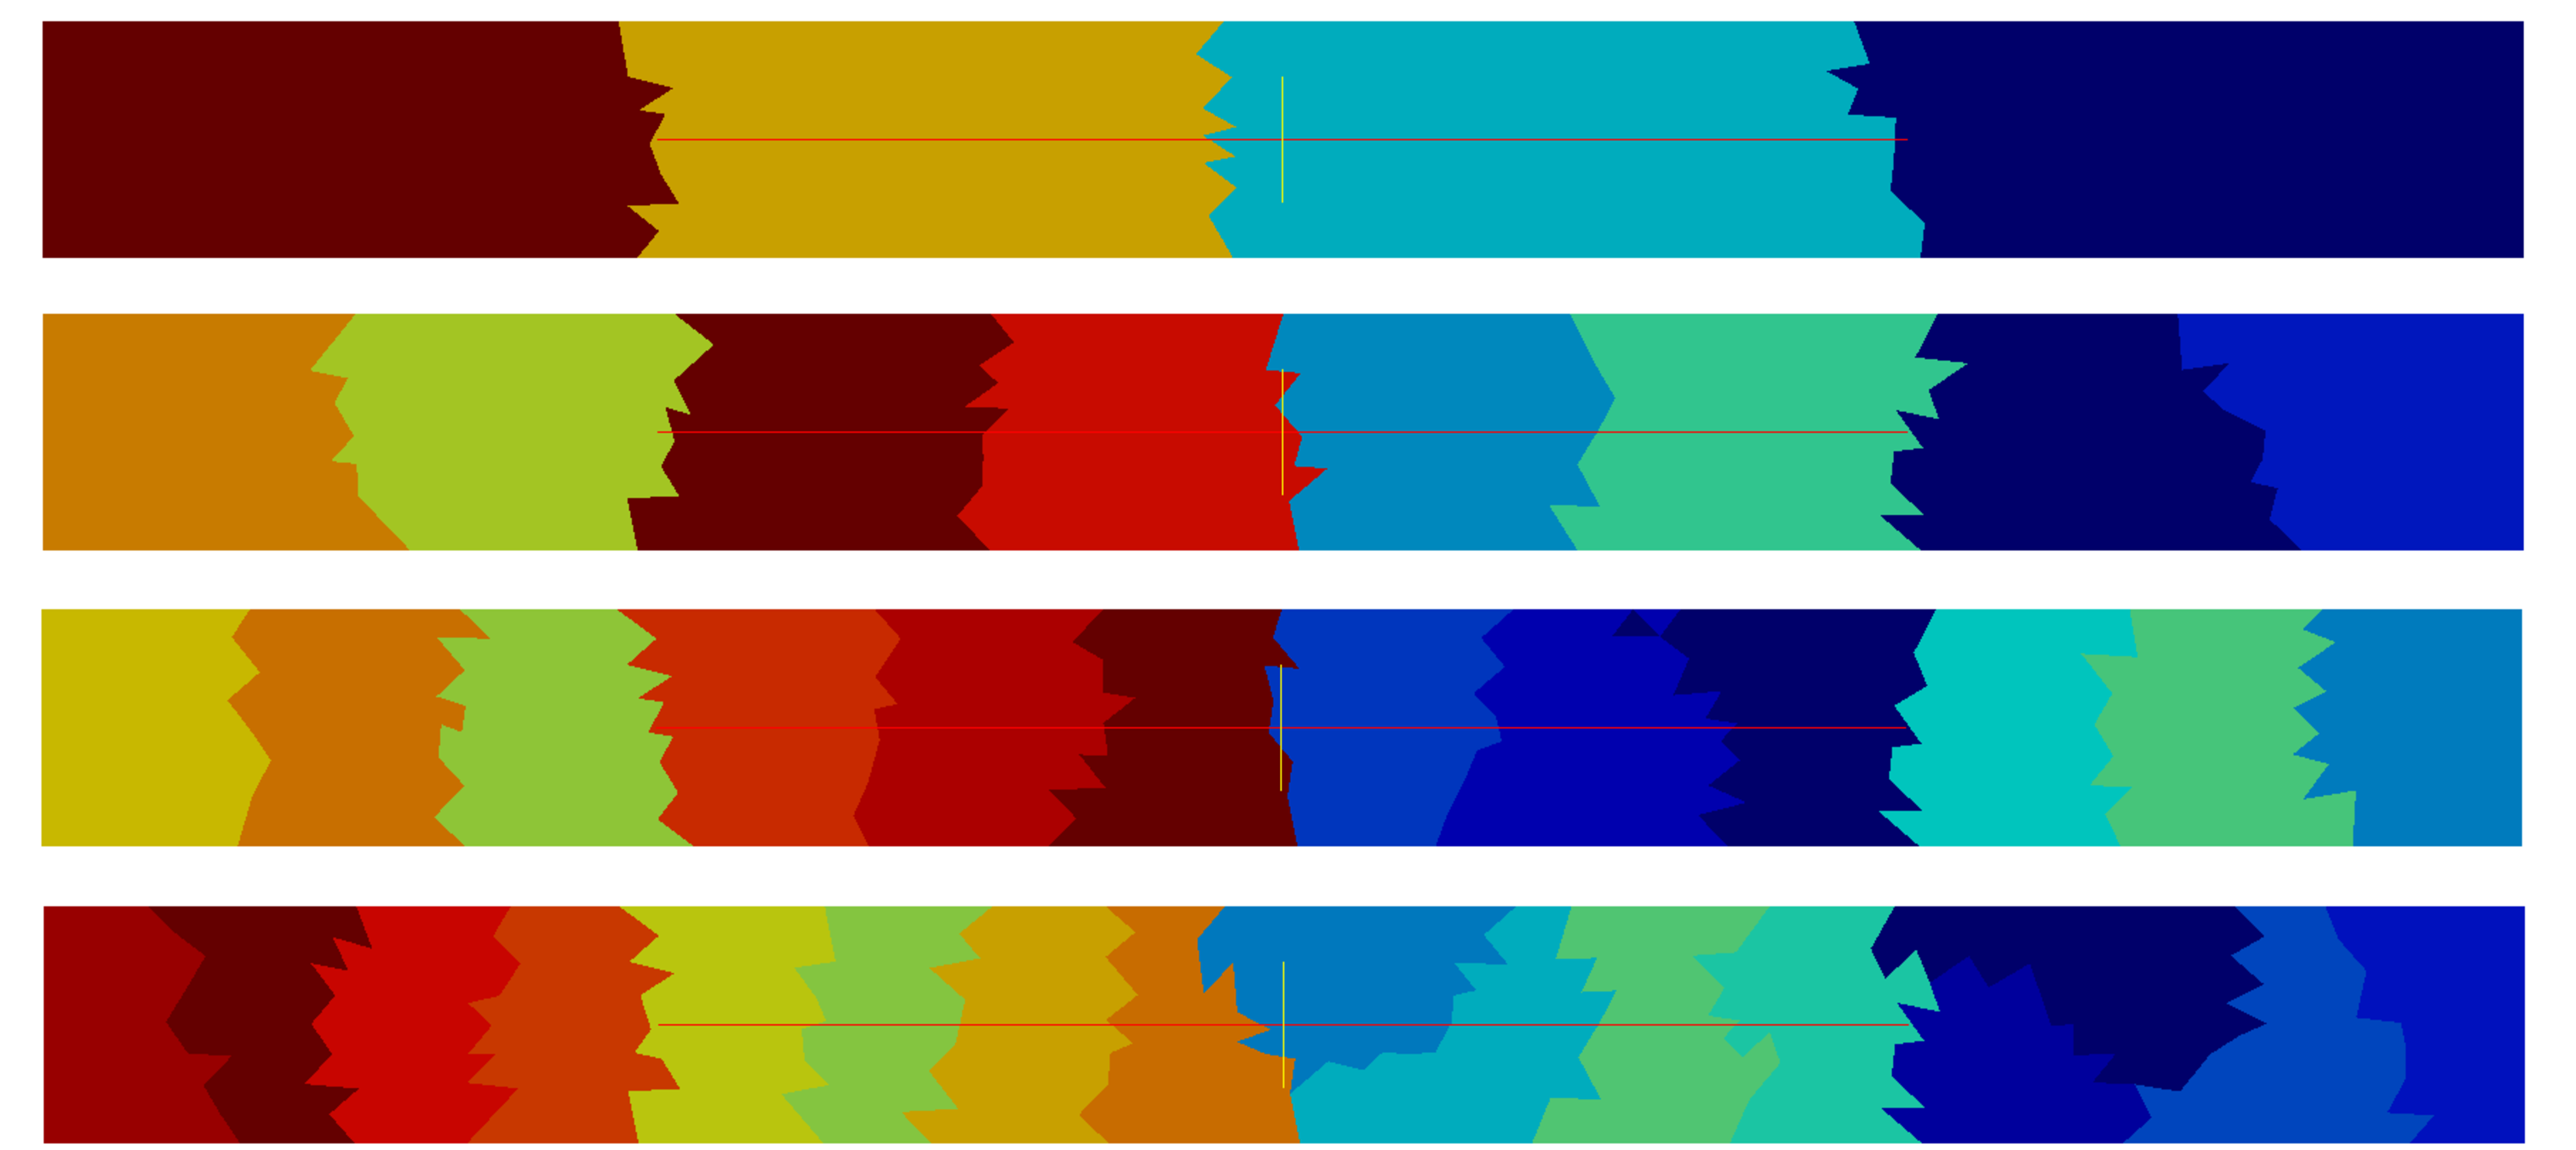
\includegraphics[width=\textwidth]{Partitions}
\caption{Rectangular waveguide partitionned in 4, 8, 12 and 16 subdomains with Metis.}
\label{fig:Partitions}
\end{figure}

The convergence histories for a 10~GHz excitations are shown in Fig. \ref{fig:DDsweep}. In the first three analyzes, an increase of the number of subdomains resulted in a slightly larger number of iterations to achieve the residual error for both solvers. In the case of 16 domains, the convergence resulted to be much harder to achieve, especially for FETI. Furthermore, in this case, the error on the scattering parameters resulted not to be bounded by the residual error as shown in table \ref{tab:SaccDDSweep}.

\begin{table}[h]
\begin{center}
\begin{tabular}{|c|c|c|}
\hline 
Solver (Nbr of Tetrahedra) & Nbr. of Sub-domains & $\frac{\Vert |S_\mathrm{ref}| - |S| \Vert_{2}}{\Vert|S_\mathrm{ref}|\Vert_2}$\\ 
\hline \hline 
\setlength{\arrayrulewidth}{0.5pt}
SCHUR (20~602) & 4 & $1.5926~10^{-6}$\\ \hline 
"& 8 & $5.95814~10^{-6}$\\ \hline 
"& 12 &  $3.29779~10^{-5}$\\ \hline 
"& 16 & $2.96923~10^{-4}$\\ \hline
FETI (20~602) & 4 & $2.14849~10^{-6}$\\ \hline 
"& 8  & $5.48124~10^{-6}$\\ \hline 
"& 12 & $1.02953~10^{-5}$\\ \hline 
"& 16 & $5.93607~10^{-3}$\\ \hline
SCHUR (25~093) & 16 & $8.29628~10^{-6}$\\ \hline 
FETI (25~093) & 16 & $1.90617~10^{-6}$\\ \hline 
\end{tabular}
\end{center}
\caption{Scattering parameters accuracy for different prescribed residual errors (runs at 10~GHz) when edge corners are avoided.}
\label{tab:SaccDDSweep}
\end{table}

The slower convergence is mainly associated to the fact there exist some edges of the mesh shared by multiple subdomains. In fact, slightly increasing the number of tetrahedra, from 20,602 to 25,093, and partitioning the new mesh in 16 subdomains without \quotes{edge corners} (Fig. \ref{fig:Partitions2}) has led to a significantly better behavior (Fig. \ref{fig:DD16ref}). Furthermore, the residual error bound could be projected, as empirically found in the previous analyzes, on the scattering parameters.

\begin{figure}[h!]
\centering
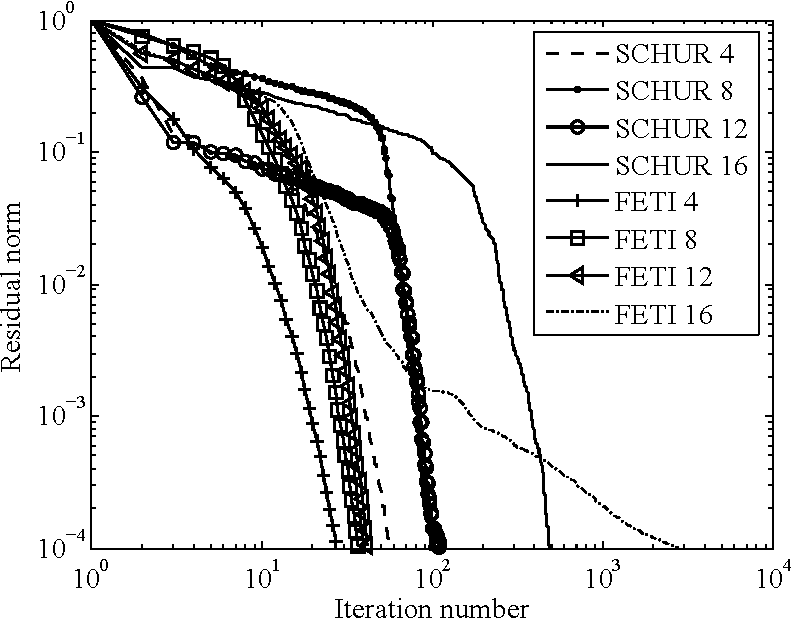
\includegraphics[width=13.4cm]{DDsweep}
\caption{Convergence histories for SCHUR and FETI GMRES(100) solvers as the number of subdomains is increased, respectively to TFE and DOM full analyzes at 10~GHz on relative mesh.}
\label{fig:DDsweep}
\end{figure}

\begin{figure}[h!]
\centering
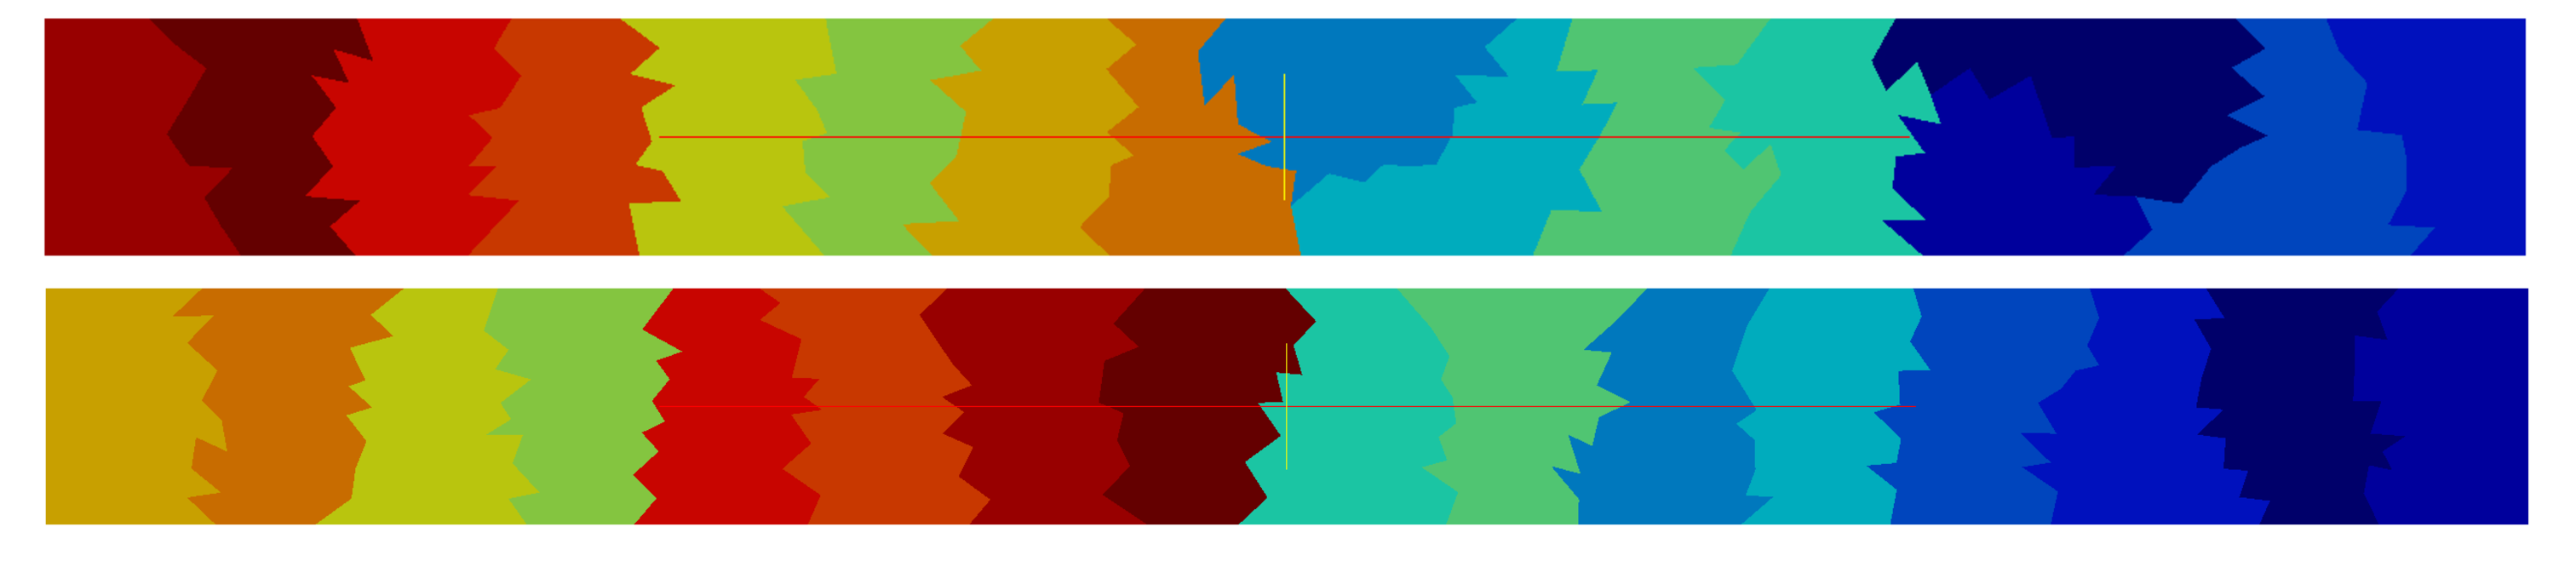
\includegraphics[width=\textwidth]{Partitions2}
\caption{The two different meshes of the rectangular waveguide both partitioned in 16 subdomains. Top to bottom: 20,602 and 25,093 tetrahedra.}
\label{fig:Partitions2}
\end{figure}

\begin{figure}[h!]
\centering
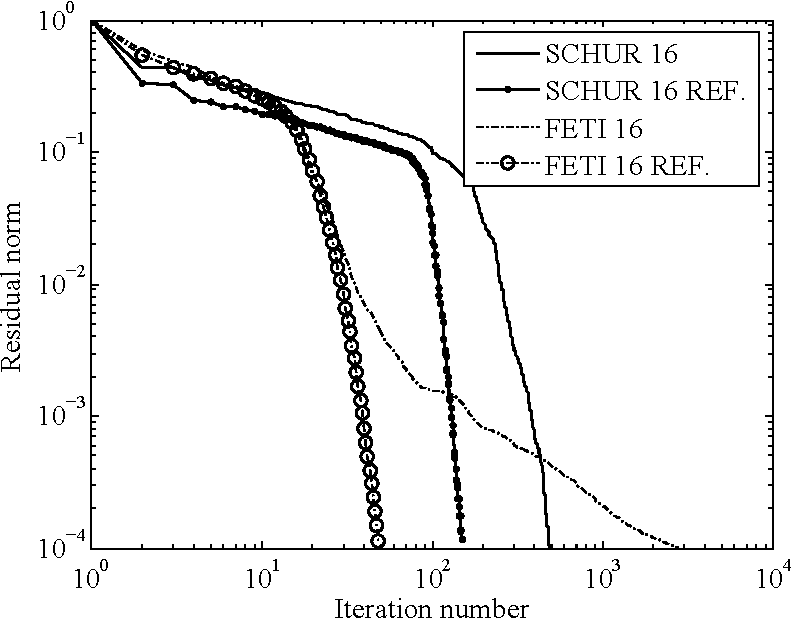
\includegraphics[width=13.4cm]{DD16ref}
\caption{Convergence histories for SCHUR and FETI GMRES(100) solvers on initial (20,602 tetrahedra) and refined (25,093 tetrahedra) meshes partitioned in 16 subdomains.}
\label{fig:DD16ref}
\end{figure}

In the average, increasing the number of subdomains on a given mesh leads to slower convergence. When partitioning the mesh, edge corners must be avoided for reliable analysis, until some solution is found to remove their bad contribution.

\subsubsection{Performances against problem size}

Although the electrical size remains the same (same structure at 10~GHz), let us analyze the performances of the solvers while increasing the mesh density and hence the number of unknowns, in order to evaluate their overall complexities. The simulations are run on a workstation equipped with an Intel Xeon CPU E5-1607 3~GHz 4 cores CPU and 64~GB of physical memory. The plots for several runs on the previous WR-90 waveguide are shown in Figs. \ref{fig:DirectCompl} and \ref{fig:IterCompl}.

\begin{figure}[h!]
\centering
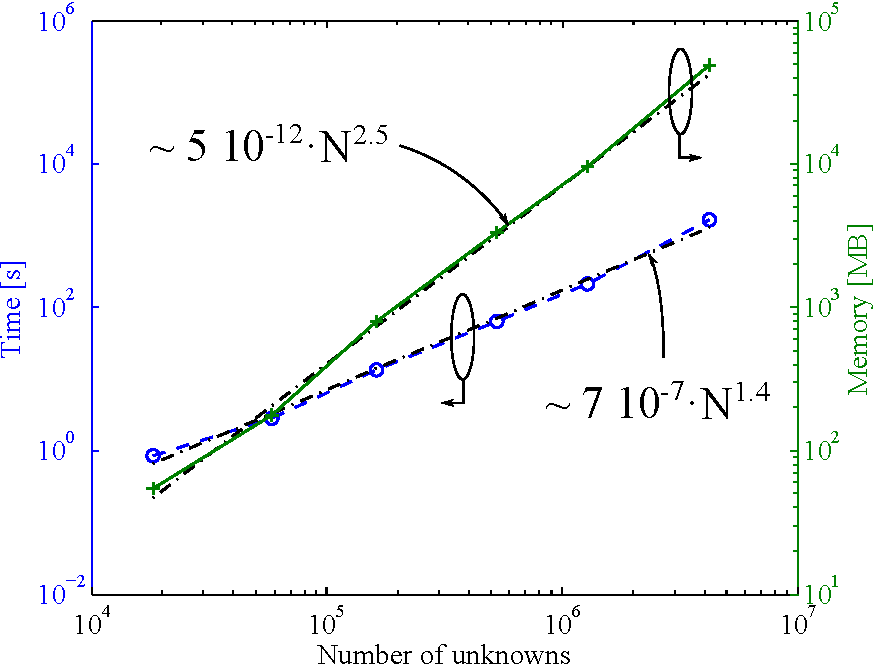
\includegraphics[width=13.4cm]{DirectCompl}
\caption{CPU time and memory consumption for different problem sizes analyzed with FES employing the double precision sparse direct solver.}
\label{fig:DirectCompl}
\end{figure}

\begin{figure}[h!]
\centering
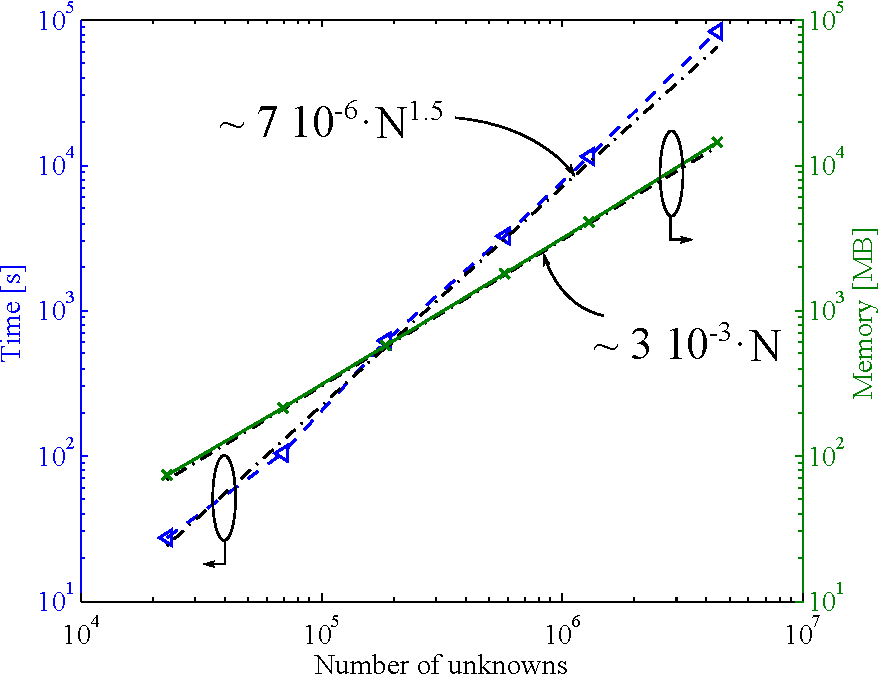
\includegraphics[width=13.4cm]{IterCompl}
\caption{CPU time and memory consumption for different problem sizes analyzed with FES employing the GMRES(100) FETI-DP preconditioned solver.}
\label{fig:IterCompl}
\end{figure}

The direct solver has a complexity of about $O(N^{2.5})$ in terms of memory, which agrees with what was stated in chapter \ref{chap:INT}, and the CPU times scale almost with an $O(N^{1.4})$ complexity. The GMRES(100) solver, FETI-DP preconditioned with the maximum number of partitions without edge corners formation and residual error of $10^{-4}$, fundamentally scales linearly in terms of memory ($O(N)$) and the times behave as $O(N^{1.5})$. It is worth noticing that while the direct solver totally exploits all the 4 cores of the CPU on which the simulations are run, the GMRES does not totally and only the sequential preconditioning does on each subdomain. Also, in the last simulation of 4.3 millions of unknowns, the direct solver required 48~GB of memory while the iterative solver on 14~GB, and hence a four times larger problem (16 millions of unknowns) could be solved on the same workstation.

%\subsection{Frequency selective radome-enclosed patch antennas array}
%
%
%In this last test we analyze the case of an large antenna problem to evaluate the influence of the residual error truncation on the antenna parameters.
%The structure analyzed is depicted in Fig. \ref{fig:RadomeFSS}. It consists of 14 2.45~GHz coaxial fed circular patch antennas \cite{maddio2011new} disposed on a 1.6~mm-thick FR4-epoxy disc substrate ($\epsilon_r = 4.4$, $\mu_r = 1$ and $\tan \delta = 0.02$) with 225~mm of diameter ($\approx 1.84~\lambda_0$). All metallic parts are considered perfect electric conductors. The enclosing radome is composed of an half sphere shell 2~mm-thick plexiglass substrate ($\epsilon_r = 3.4$, $\mu_r = 1$ and $\tan \delta = 0.001$) on which metallic O-rings (inner diameter of 4.2~mm and outer of 10~mm) are imprinted. The radome has me
%
%\begin{figure}[!]
%\centering
%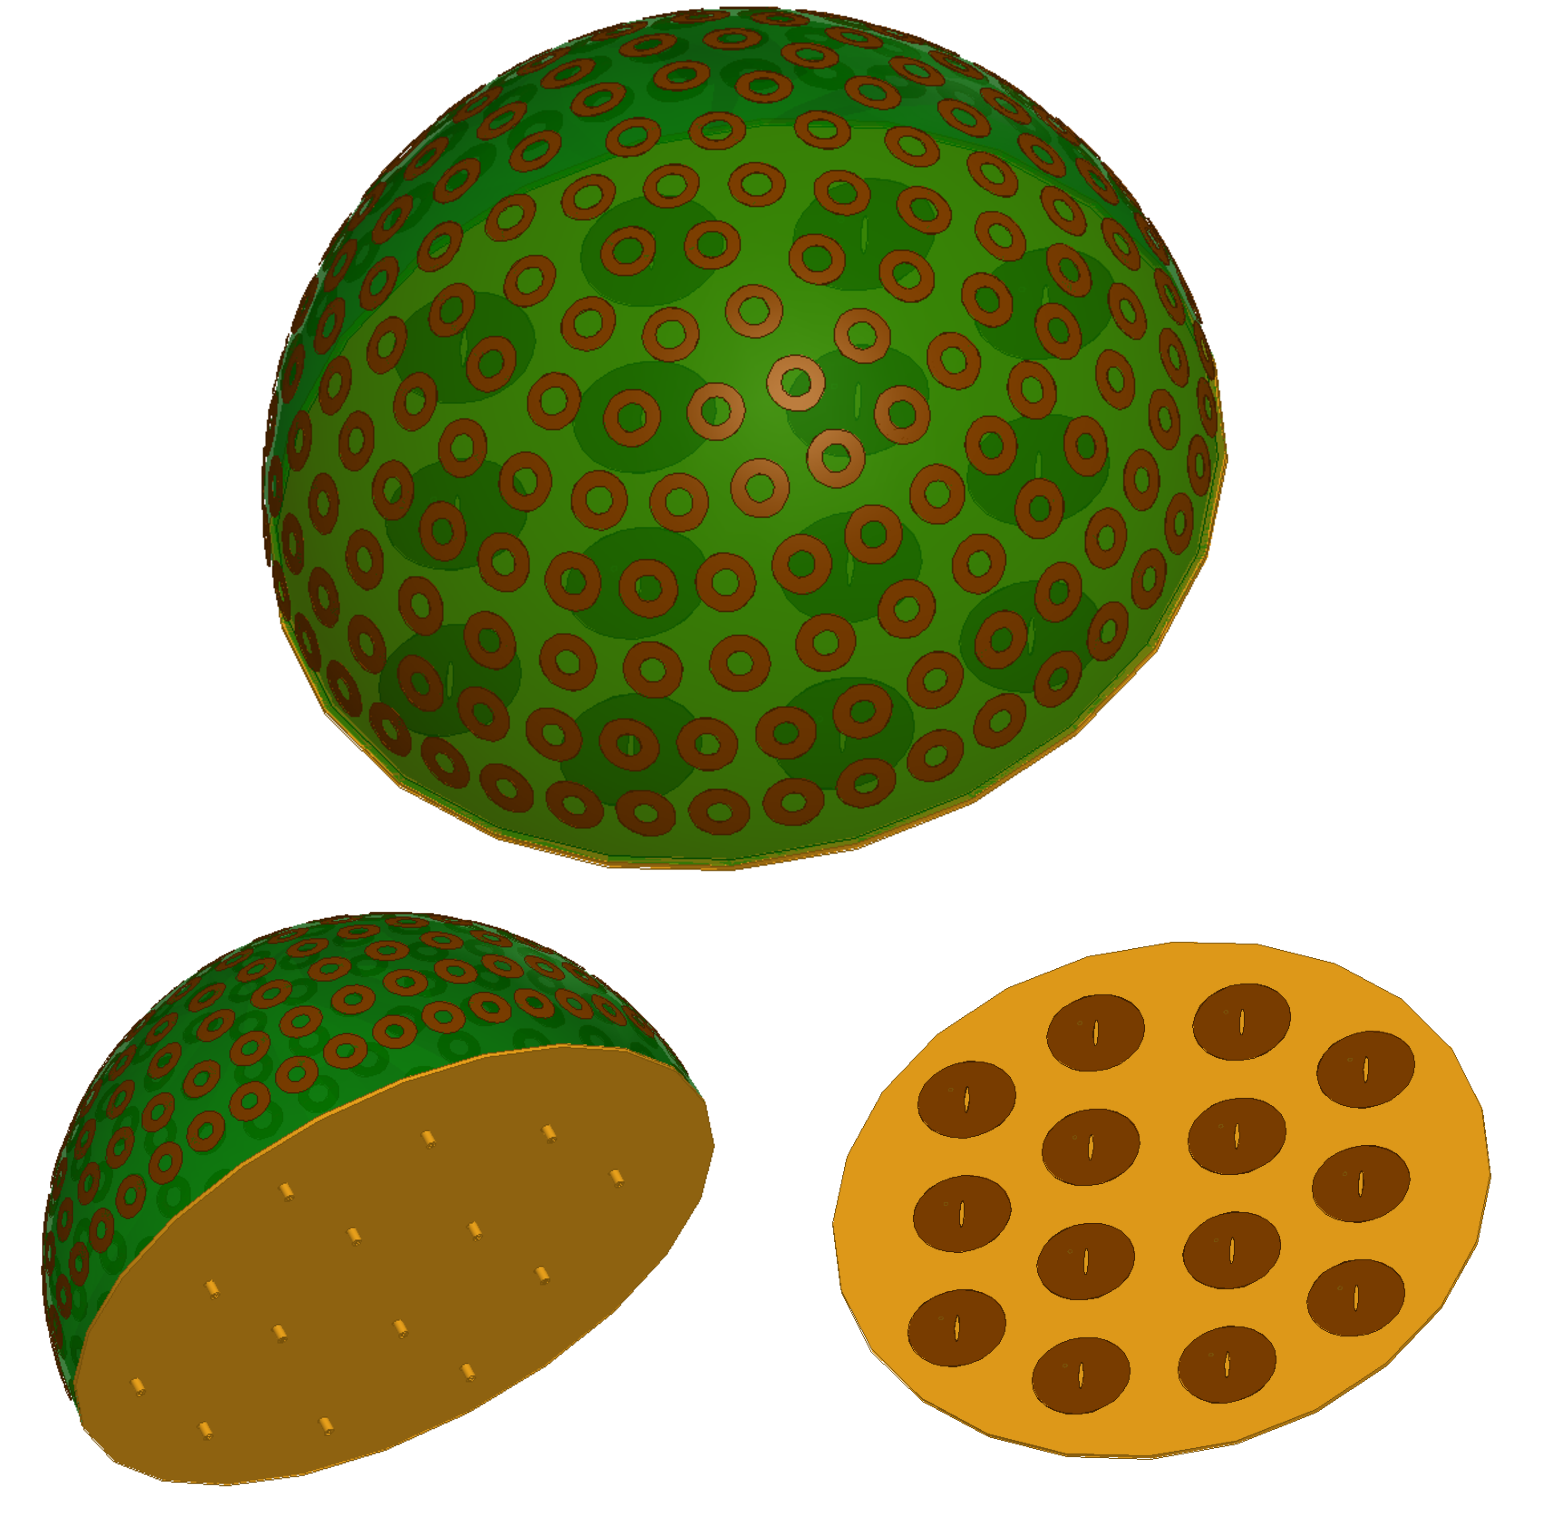
\includegraphics[width=13.4cm]{RadomeFSS}
%\caption{CAD model of the FSS radome-enclosed circular patch antenna array.}
%\label{fig:RadomeFSS}
%\end{figure}
%
%The mesh of the structure has led to almost 1~255~428 tetrahedra due to the small thicknesses of the substrate and the radome, Also, around metals the mesh density had to be increased in order to accurately approximate the large fields gradients (Fig. \ref{fig:Mesh}).
%
%\begin{figure}[!]
%\centering
%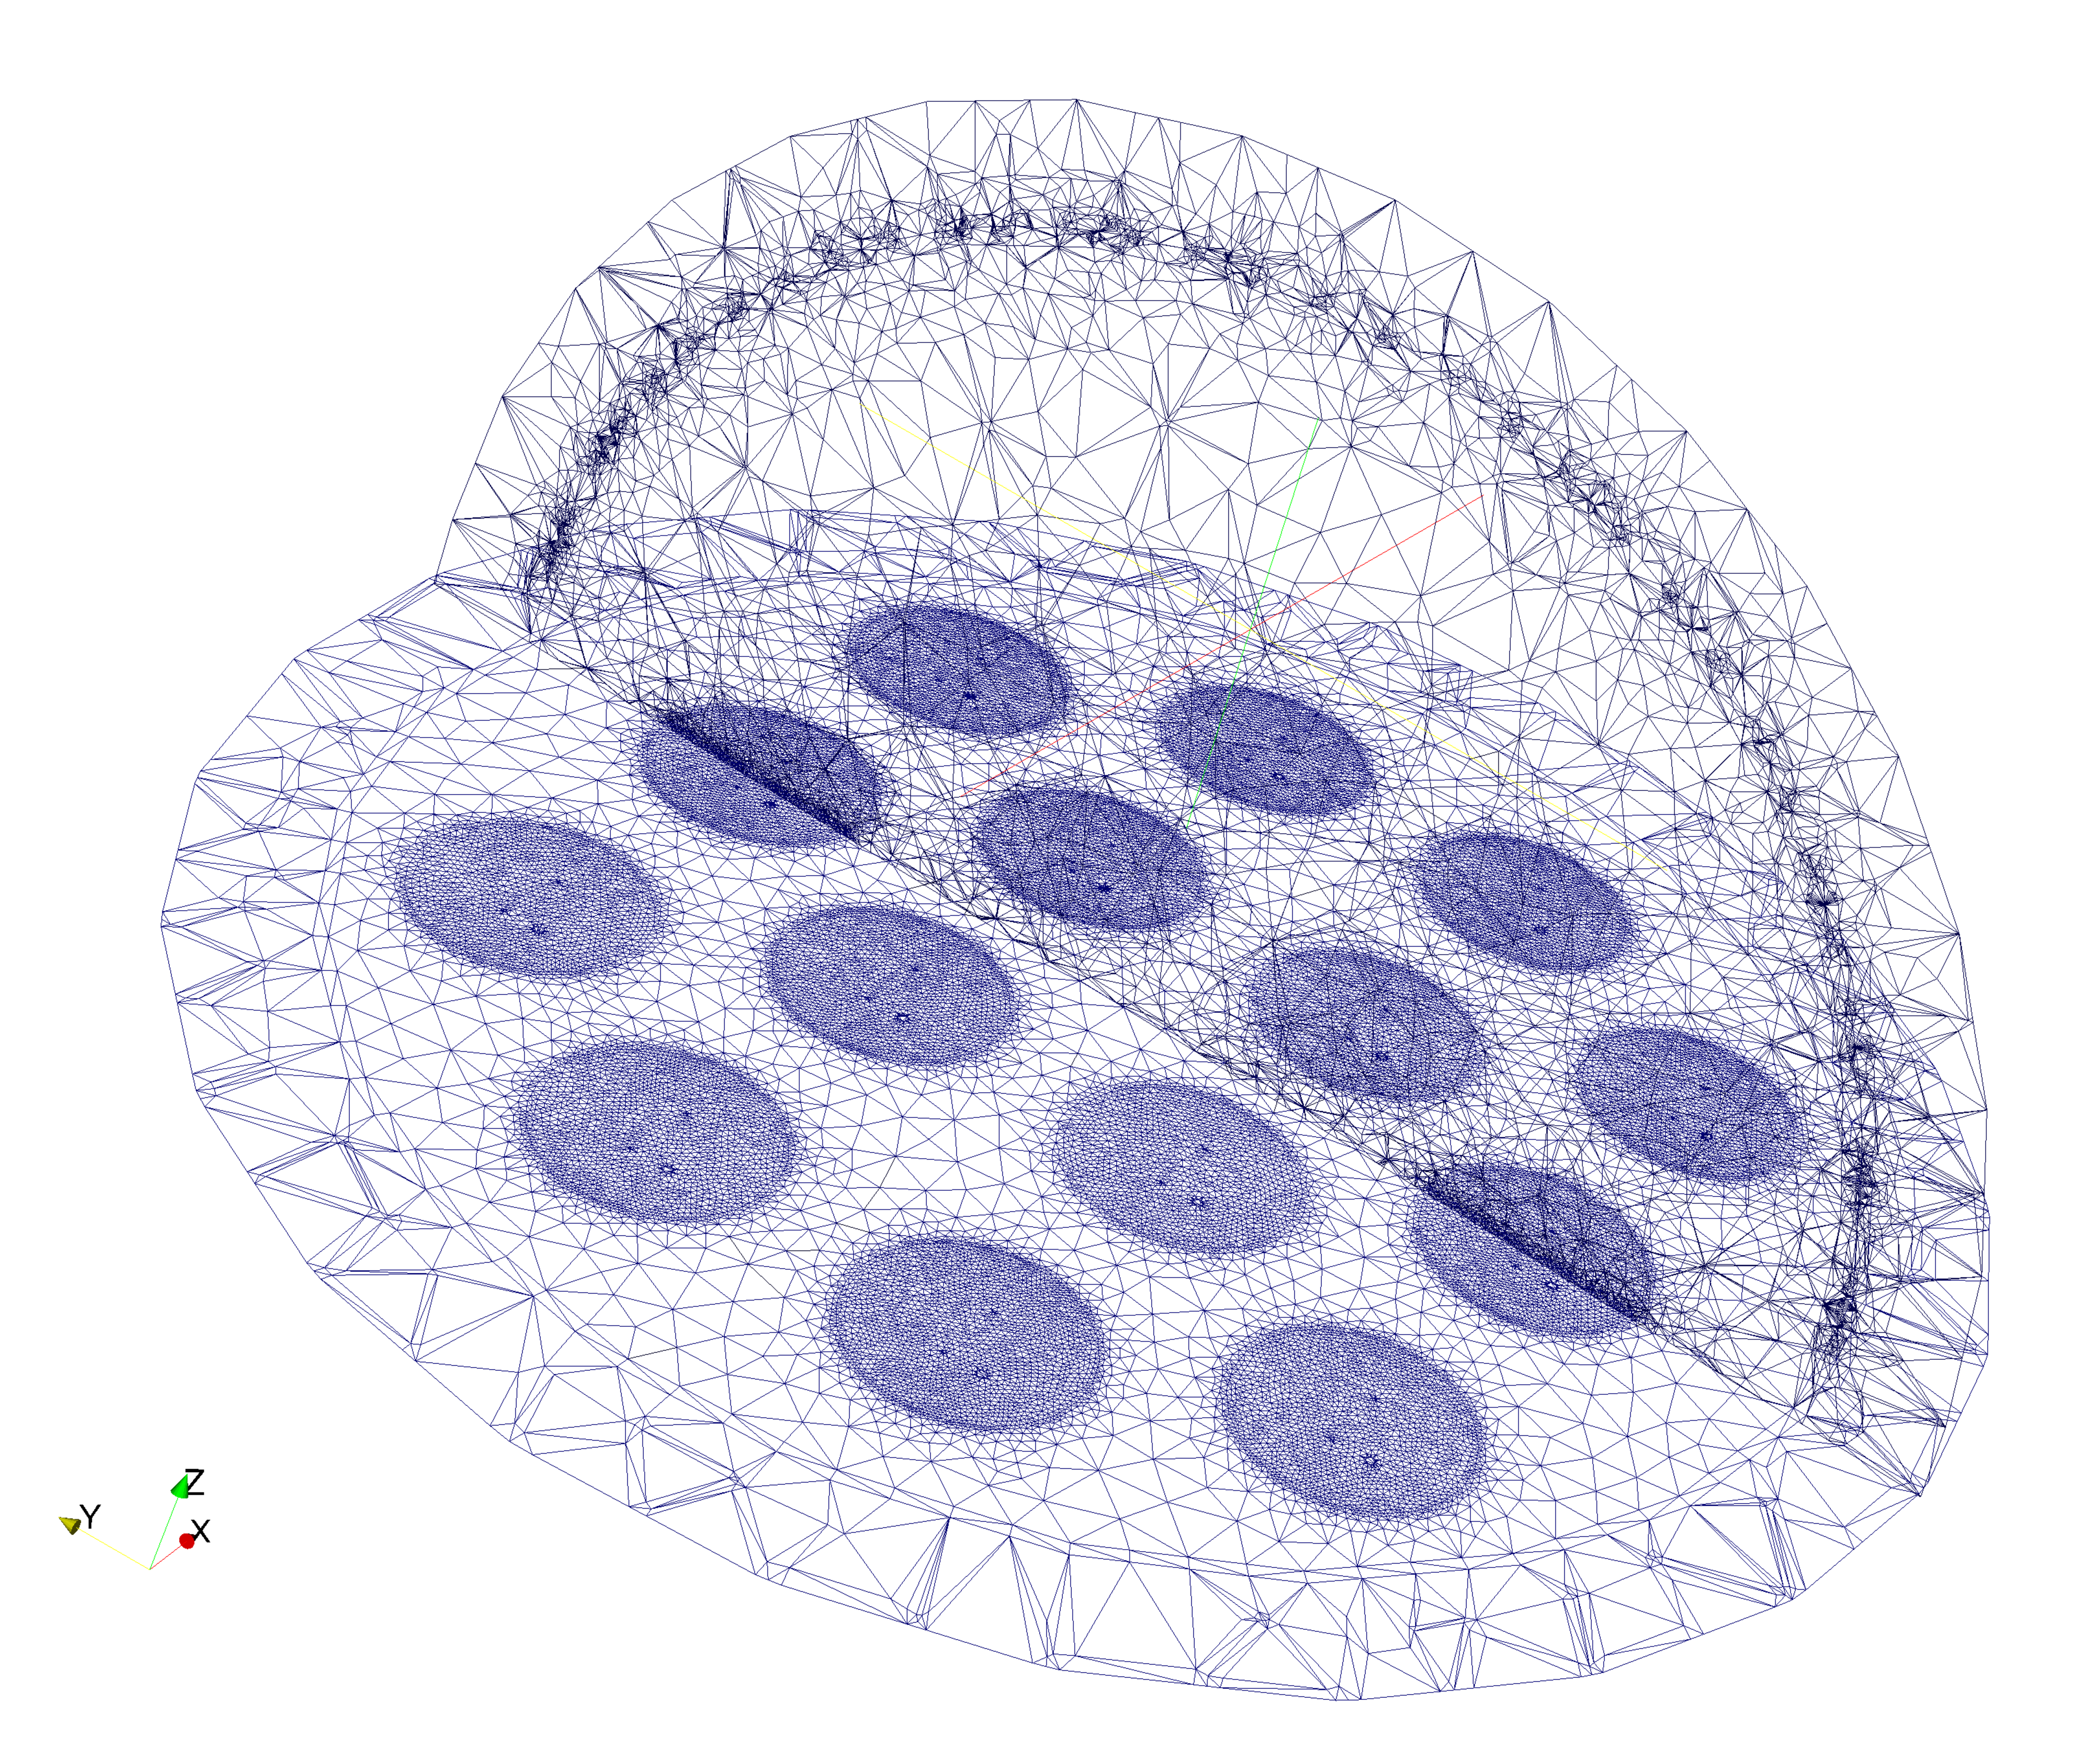
\includegraphics[width=13.4cm]{Mesh}
%\caption{Cross sections of the mesh.}
%\label{fig:Mesh}
%\end{figure}
%
%An assembly of the finite element matrices with first order curl-conforming basis functions and  has led to 1~297~027 unknowns, considering dominant, coaxial TEM mode impinging on each waveport. The radiation boundaries are located $\frac{\lambda_0}{4}$ away form the radome, on a concentric spherical shell.
